% Options for packages loaded elsewhere
\PassOptionsToPackage{unicode}{hyperref}
\PassOptionsToPackage{hyphens}{url}
\PassOptionsToPackage{dvipsnames,svgnames,x11names}{xcolor}
%
\documentclass[
  11pt,
  letterpaper,
]{article}
\usepackage{amsmath,amssymb}
\usepackage{iftex}
\ifPDFTeX
  \usepackage[T1]{fontenc}
  \usepackage[utf8]{inputenc}
  \usepackage{textcomp} % provide euro and other symbols
\else % if luatex or xetex
  \usepackage{unicode-math} % this also loads fontspec
  \defaultfontfeatures{Scale=MatchLowercase}
  \defaultfontfeatures[\rmfamily]{Ligatures=TeX,Scale=1}
\fi
\usepackage{lmodern}
\ifPDFTeX\else
  % xetex/luatex font selection
\fi
% Use upquote if available, for straight quotes in verbatim environments
\IfFileExists{upquote.sty}{\usepackage{upquote}}{}
\IfFileExists{microtype.sty}{% use microtype if available
  \usepackage[]{microtype}
  \UseMicrotypeSet[protrusion]{basicmath} % disable protrusion for tt fonts
}{}
\makeatletter
\@ifundefined{KOMAClassName}{% if non-KOMA class
  \IfFileExists{parskip.sty}{%
    \usepackage{parskip}
  }{% else
    \setlength{\parindent}{0pt}
    \setlength{\parskip}{6pt plus 2pt minus 1pt}}
}{% if KOMA class
  \KOMAoptions{parskip=half}}
\makeatother
\usepackage{xcolor}
\usepackage[margin=1in]{geometry}
\usepackage{longtable,booktabs,array}
\usepackage{calc} % for calculating minipage widths
% Correct order of tables after \paragraph or \subparagraph
\usepackage{etoolbox}
\makeatletter
\patchcmd\longtable{\par}{\if@noskipsec\mbox{}\fi\par}{}{}
\makeatother
% Allow footnotes in longtable head/foot
\IfFileExists{footnotehyper.sty}{\usepackage{footnotehyper}}{\usepackage{footnote}}
\makesavenoteenv{longtable}
\usepackage{graphicx}
\makeatletter
\def\maxwidth{\ifdim\Gin@nat@width>\linewidth\linewidth\else\Gin@nat@width\fi}
\def\maxheight{\ifdim\Gin@nat@height>\textheight\textheight\else\Gin@nat@height\fi}
\makeatother
% Scale images if necessary, so that they will not overflow the page
% margins by default, and it is still possible to overwrite the defaults
% using explicit options in \includegraphics[width, height, ...]{}
\setkeys{Gin}{width=\maxwidth,height=\maxheight,keepaspectratio}
% Set default figure placement to htbp
\makeatletter
\def\fps@figure{htbp}
\makeatother
\setlength{\emergencystretch}{3em} % prevent overfull lines
\providecommand{\tightlist}{%
  \setlength{\itemsep}{0pt}\setlength{\parskip}{0pt}}
\setcounter{secnumdepth}{-\maxdimen} % remove section numbering
% definitions for citeproc citations
\NewDocumentCommand\citeproctext{}{}
\NewDocumentCommand\citeproc{mm}{%
  \begingroup\def\citeproctext{#2}\cite{#1}\endgroup}
\makeatletter
 % allow citations to break across lines
 \let\@cite@ofmt\@firstofone
 % avoid brackets around text for \cite:
 \def\@biblabel#1{}
 \def\@cite#1#2{{#1\if@tempswa , #2\fi}}
\makeatother
\newlength{\cslhangindent}
\setlength{\cslhangindent}{1.5em}
\newlength{\csllabelwidth}
\setlength{\csllabelwidth}{3em}
\newenvironment{CSLReferences}[2] % #1 hanging-indent, #2 entry-spacing
 {\begin{list}{}{%
  \setlength{\itemindent}{0pt}
  \setlength{\leftmargin}{0pt}
  \setlength{\parsep}{0pt}
  % turn on hanging indent if param 1 is 1
  \ifodd #1
   \setlength{\leftmargin}{\cslhangindent}
   \setlength{\itemindent}{-1\cslhangindent}
  \fi
  % set entry spacing
  \setlength{\itemsep}{#2\baselineskip}}}
 {\end{list}}
\usepackage{calc}
\newcommand{\CSLBlock}[1]{\hfill\break\parbox[t]{\linewidth}{\strut\ignorespaces#1\strut}}
\newcommand{\CSLLeftMargin}[1]{\parbox[t]{\csllabelwidth}{\strut#1\strut}}
\newcommand{\CSLRightInline}[1]{\parbox[t]{\linewidth - \csllabelwidth}{\strut#1\strut}}
\newcommand{\CSLIndent}[1]{\hspace{\cslhangindent}#1}
\ifLuaTeX
  \usepackage{selnolig}  % disable illegal ligatures
\fi
\usepackage{bookmark}
\IfFileExists{xurl.sty}{\usepackage{xurl}}{} % add URL line breaks if available
\urlstyle{same}
\hypersetup{
  pdftitle={Quantum Technologies as Strategic Infrastructure: Evidence, Adoption Pathways, and a National Research Agenda for 2025-2035},
  pdfauthor={Edgar Valdés, Hadox Research Labs},
  colorlinks=true,
  linkcolor={blue},
  filecolor={blue},
  citecolor={blue},
  urlcolor={blue},
  pdfcreator={LaTeX via pandoc}}

\title{Quantum Technologies as Strategic Infrastructure: Evidence,
Adoption Pathways, and a National Research Agenda for
2025-2035\thanks{Prepared for the Quantum Technologies track of the
twenty-third edition of the Global Information Technology Management
Association Annual Conference, Monterrey, Mexico, May 6-8, 2026, for
which Edgar Antonio Valdés Porras serves as Track Chair. The author
gratefully acknowledges Rogelio Marín and the Centro de Investigación en
Matemáticas, A.C. for intellectual support and institutional context.
All interpretations and remaining errors are the author's
responsibility.}}
\author{Edgar Valdés, Hadox Research Labs}
\date{April 2026}

\begin{document}
\maketitle

\section{Abstract}\label{abstract}

Quantum technologies have moved from a predominantly scientific
programme into a strategic infrastructure domain affecting computation,
sensing, communications, cybersecurity, industrial research, and
national innovation policy. The 2025-2035 adoption horizon is examined
through an integrative synthesis of the quantum information science
literature, innovation systems theory, enterprise-adoption research,
OECD national strategy data, OECD-EPO patent mapping, OpenAlex
bibliometric indicators, NIST standards, high-performance computing
(HPC) integration studies, and public readiness surveys. The analysis
finds that quantum adoption is not a single market transition but a
layered capability transition: post-quantum cryptography and selected
quantum sensing applications already have institutional relevance;
quantum communication develops through specialized network and security
testbeds; and general-purpose quantum computing remains contingent on
error correction, logical-qubit economics, application-level
benchmarking, hybrid quantum-classical integration, and the ability to
couple quantum processing units to HPC environments. The empirical
record shows acceleration as well as structural unevenness. Governments
had announced approximately USD 55.7 billion in quantum commitments by
October 2025; OECD Fundstat identified USD 11.235 billion PPP in 12,209
quantum-related R\&D awards during 2015-2023; OECD-EPO mapping
identified 31,700 quantum patent families from 2005-2024; and OpenAlex
bibliometrics show a publication geography concentrated in the United
States, China, Germany, the United Kingdom, and France. These findings
support a shift from hardware-centered readiness metrics toward
absorptive capacity: the capacity of firms and states to understand,
test, benchmark, procure, secure, regulate, and eventually produce
quantum technologies. The article concludes with a staged roadmap, a
critique of common adoption errors, and a frontier research agenda for
nations seeking long-term technological sovereignty.

\textbf{Keywords:} quantum technologies, quantum computing, quantum
sensing, post-quantum cryptography, quantum communication, national
innovation systems, absorptive capacity, quantum policy, strategic
infrastructure

\section{1. Introduction}\label{introduction}

The term ``quantum technology'' now carries two different meanings. In
public discourse it is often used as a synonym for quantum computing,
accompanied by claims that quantum processors will soon transform every
computational problem. In the research literature it denotes a broader
family of technologies that exploit controlled quantum states for
computation, measurement, communication, simulation, timing, and
security (\citeproc{ref-dowling2003}{Dowling and Milburn 2003};
\citeproc{ref-acin2018}{Acin et al. 2018}). This distinction is
analytically consequential because it changes how adoption, policy,
investment, and national strategy are evaluated.

The first quantum revolution produced technologies such as transistors,
lasers, magnetic resonance imaging, semiconductor electronics, and
atomic clocks. These devices used quantum theory indirectly, often
through bulk or statistical properties of matter. The second quantum
revolution is different because it seeks direct engineering of
individual or collective quantum states, including superposition,
entanglement, squeezing, tunneling, and measurement back-action
(\citeproc{ref-dowling2003}{Dowling and Milburn 2003};
\citeproc{ref-giovannetti2011}{Giovannetti, Lloyd, and Maccone 2011}).
Quantum technologies therefore sit at the boundary between physics and
infrastructure. They are scientific instruments, but they are also
future components of cybersecurity, finance, telecommunications, energy,
medicine, logistics, materials discovery, defense, and public
administration.

The analysis treats quantum technologies as strategic infrastructure.
That framing has three implications. First, quantum technologies are not
a single product market. They form a stack of scientific, industrial,
software, security, metrology, and governance capabilities. Second,
their economic value will not be captured simply by the earliest vendors
or by the largest hardware announcements. It will be captured by
organizations and countries that develop the capacity to evaluate
quantum claims, integrate quantum tools with classical systems, and
adapt procurement, standards, talent, and cybersecurity. Third, the most
important near-term actions are not always those that sound most
futuristic. Post-quantum cryptography (PQC), quantum-safe procurement,
quantum sensing pilots, metrology, workforce formation, and
cloud-mediated experimentation may produce more strategic value before
universal fault-tolerant quantum computing arrives.

Five research questions structure the analysis.

\begin{enumerate}
\def\labelenumi{\arabic{enumi}.}
\tightlist
\item
  What does the scholarly literature imply about the maturity and
  adoption pathways of quantum computing, sensing, communication, and
  post-quantum cryptography?
\item
  What quantitative indicators can be used to estimate global quantum
  readiness when direct adoption data remain incomplete?
\item
  How does high-performance computing change the adoption pathway for
  quantum computing?
\item
  How can nations and enterprises compare quantum technologies under
  conditions of technical uncertainty, hype, and geopolitical
  competition?
\item
  What are the principal barriers to quantum adoption between 2025 and
  2035?
\item
  What roadmap can guide a nation toward quantum capability without
  premature lock-in to immature hardware or rhetorical innovation
  policy?
\end{enumerate}

The argument is intentionally critical. Quantum technologies are real
and strategically important, but their adoption is often discussed with
weak evidence. Market forecasts can be useful signals, but they are not
adoption data. Qubit counts are not system capability. Random-circuit
advantage is not automatically commercial value. Quantum key
distribution is not a universal replacement for post-quantum
cryptography. Quantum machine learning is not automatically superior to
classical machine learning. A credible national strategy requires clear
separation among scientific possibility, engineering feasibility,
organizational readiness, and public value.

\section{2. Literature Review and Theoretical
Frame}\label{literature-review-and-theoretical-frame}

\subsection{2.1 From Quantum Revolution to
Infrastructure}\label{from-quantum-revolution-to-infrastructure}

The modern quantum technology agenda begins with the claim that
individual quantum systems can be engineered as resources rather than
treated as unavoidable microscopic phenomena. Dowling and Milburn
(\citeproc{ref-dowling2003}{2003}) described this as the second quantum
revolution. The European quantum roadmap later organized the field into
quantum communication, quantum computation, quantum simulation, quantum
metrology and sensing, quantum control, and quantum software
(\citeproc{ref-acin2018}{Acin et al. 2018}). This taxonomy remains
useful, but national strategy requires an additional classification by
adoption readiness, infrastructure burden, security urgency, and
dependence on fault tolerance.

Quantum computing receives the most attention because its long-run
computational implications are profound. Montanaro
(\citeproc{ref-montanaro2016}{2016}) shows that quantum algorithms can
offer speedups in areas such as search, optimization, simulation, linear
systems, and cryptography. Preskill (\citeproc{ref-preskill2018}{2018})
framed the present era as noisy intermediate-scale quantum computing, in
which devices are large enough to be scientifically interesting but too
noisy for many fault-tolerant algorithms. Bharti et al.
(\citeproc{ref-bharti2022}{2022}) and Cerezo et al.
(\citeproc{ref-cerezo2021}{2021}) show that the near-term algorithmic
landscape is dominated by variational and hybrid quantum-classical
methods, not by the mature execution of Shor-scale fault-tolerant
algorithms. This matters because the route from laboratory device to
operational advantage is not a straight line; it runs through error
correction, benchmark design, software tooling, and application-specific
validation.

Quantum simulation and quantum chemistry provide the clearest
intellectual case for future quantum computation because the target
systems are themselves quantum mechanical. Georgescu, Ashhab, and Nori
(\citeproc{ref-georgescu2014}{2014}) present quantum simulation as a
natural application class, while Cao et al.
(\citeproc{ref-cao2019}{2019}) and Bauer et al.
(\citeproc{ref-bauer2020}{2020}) review algorithms for chemistry and
materials science. Yet even here the adoption problem is not solved by
theoretical advantage. Useful workflows require chemical accuracy,
problem encoding, error mitigation or correction, validation against
experiments, and integration into existing research pipelines.

Quantum sensing follows a different path. Degen, Reinhard, and
Cappellaro (\citeproc{ref-degen2017}{2017}) define quantum sensing as
the use of quantum systems to measure physical quantities with high
sensitivity. Giovannetti, Lloyd, and Maccone
(\citeproc{ref-giovannetti2011}{2011}) and Pezze et al.
(\citeproc{ref-pezze2018}{2018}) show why entanglement and nonclassical
states can improve metrology. Applications such as clocks,
magnetometers, gravimeters, inertial sensors, navigation, geodesy, and
biomedical sensing do not require universal fault-tolerant quantum
computation. This makes sensing a nearer-term adoption domain, although
the engineering requirements remain demanding: ruggedization,
calibration, cost, environmental stability, field deployment, and
integration into domain workflows.

Quantum communication also has a distinct maturity profile. Kimble
(\citeproc{ref-kimble2008}{2008}) and Wehner, Elkouss, and Hanson
(\citeproc{ref-wehner2018}{2018}) describe the quantum internet as a
future network for entanglement distribution, secure communication,
distributed sensing, and eventually distributed quantum computation.
Pirandola et al. (\citeproc{ref-pirandola2020}{2020}) and Xu et al.
(\citeproc{ref-xu2020}{2020}) review quantum cryptography and QKD with
realistic devices. The research case is strong, but practical deployment
faces distance limits, loss, authentication, trusted nodes, device
vulnerabilities, cost, and standards. The result is a specialized
infrastructure pathway rather than a universal cybersecurity solution.

PQC is conceptually different from quantum communication. It is
classical cryptography designed to resist quantum attacks. Bernstein and
Lange (\citeproc{ref-bernstein2017}{2017}) review the technical
foundations of post-quantum cryptography; Mosca
(\citeproc{ref-mosca2018}{2018}) frames the cybersecurity problem
through the relation between data shelf life, migration time, and the
timeline for cryptographically relevant quantum computers. Gidney and
Ekera (\citeproc{ref-gidney2021}{2021}) show why the threat is not
imminent in an operational sense but is strategically serious: resource
estimates for attacking RSA-2048 require very large fault-tolerant
machines, yet the ``harvest now, decrypt later'' problem begins before
those machines exist. This makes PQC the clearest near-term national
adoption domain.

\subsection{2.2 Adoption Theory: Absorptive Capacity and National
Innovation
Systems}\label{adoption-theory-absorptive-capacity-and-national-innovation-systems}

Quantum adoption is not only a hardware problem. It is an absorptive
capacity problem. Cohen and Levinthal (\citeproc{ref-cohen1990}{1990})
define absorptive capacity as the ability to recognize, assimilate, and
exploit external knowledge. Quantum technologies require unusually high
absorptive capacity because they are difficult to evaluate, require
specialized expertise, and depend on complementary assets such as
standards, laboratories, software platforms, cryptographic inventories,
and procurement rules.

National innovation systems theory reinforces this point. Technological
performance depends on networks of universities, firms, public agencies,
standards bodies, financial institutions, and industrial users rather
than isolated inventions (\citeproc{ref-lundvall1992}{Lundvall 1992};
\citeproc{ref-nelson1993}{Nelson 1993}). Mission-oriented innovation
policy adds that governments can shape markets when they define public
missions, coordinate capabilities, and create demand for difficult
technologies (\citeproc{ref-mazzucato2018}{Mazzucato 2018}). Quantum
technologies fit this framework because the private sector alone is
unlikely to fund all foundational science, cybersecurity transition,
standards, workforce development, and testbed infrastructure required
for adoption.

Enterprise adoption evidence is beginning to catch up with the physics.
Kwon et al. (\citeproc{ref-kwon2026}{2026}) analyze quantum computing
adoption intention through expert interviews and a survey of 250 IT
decision-makers. They find that perceived quantum advantage, belief in
quantum superiority, continuous budget allocation, regulatory support,
and co-creation increase adoption intention, while organizational
resistance and financial risk reduce it. The result is consistent with
the broader innovation diffusion literature: adoption requires not just
technological promise but relative advantage, compatibility,
trialability, organizational resources, and institutional support
(\citeproc{ref-rogers2003}{Rogers 2003}).

\subsection{2.3 The Strategic Error: Confusing Scientific Milestones
with
Adoption}\label{the-strategic-error-confusing-scientific-milestones-with-adoption}

The quantum field has produced genuine scientific milestones. Arute et
al. (\citeproc{ref-arute2019}{2019}) demonstrated quantum computational
advantage on a programmable superconducting processor for a sampling
task. Harrow and Montanaro (\citeproc{ref-harrow2017}{2017}) explain why
such demonstrations matter for computational complexity. However,
scientific advantage and economic advantage are not the same. A
random-circuit sampling task can demonstrate that a quantum device is
difficult to simulate classically without solving a valuable business
problem. This is not a criticism of the science; it is a warning against
using the wrong inference for policy.

The same distinction applies to quantum machine learning. Biamonte et
al. (\citeproc{ref-biamonte2017}{2017}) and Schuld and Killoran
(\citeproc{ref-schuld2019}{2019}) identify plausible quantum machine
learning mechanisms, especially through feature maps and Hilbert-space
representations. McClean et al. (\citeproc{ref-mcclean2018}{2018}),
however, identify barren plateaus as a serious training obstacle. For
enterprise strategy, the relevant question is not whether a circuit is
quantum, but whether it improves accuracy, time-to-solution, energy
consumption, robustness, interpretability, or cost relative to the best
classical baseline.

\section{3. Data and Methods}\label{data-and-methods}

\subsection{3.1 Research Design}\label{research-design}

The study is designed as an integrative research synthesis. This design
is appropriate because the object of inquiry is not a single empirical
estimate but a strategic interpretation of a heterogeneous evidence
base. The evidentiary corpus includes quantum information science,
innovation theory, policy reports, open bibliometric data, patent
mapping, standards documents, and business-readiness surveys.

The methodology follows four steps. First, the literature was organized
into seven domains: quantum computing, quantum sensing, quantum
communication, PQC, high-performance computing integration,
innovation/adoption theory, and national policy. Second, each domain was
evaluated according to technology readiness, adoption barriers,
infrastructure requirements, and relevance to national strategy. Third,
quantitative adoption proxies were assembled from OECD, OECD-EPO,
OpenAlex, NIST, and readiness survey sources.\footnote{Adoption proxies
  are used because comprehensive public data on direct quantum
  deployment remain unavailable. They measure different dimensions of
  readiness and are not treated as interchangeable indicators.} Fourth,
the evidence was translated into a strategic roadmap and a set of
decision criteria for nations and enterprises.

The design is not a systematic review in the narrow PRISMA sense, since
the objective is not to estimate an effect size across comparable
empirical studies. It is a structured narrative review and evidence
synthesis of an emerging technology field in which relevant evidence
comes from physics, computer science, cybersecurity, policy, and
management research. The inclusion criteria prioritized major review
articles, highly cited foundational papers, empirical adoption studies,
standards-relevant cybersecurity literature, and recent policy datasets
from public institutions.

\subsection{3.2 Source Selection}\label{source-selection}

The scholarly corpus was drawn from journals and proceedings in physics,
computer science, engineering, cryptography, management, and innovation
policy. It includes work published in \emph{Reviews of Modern Physics},
\emph{Nature}, \emph{Nature Reviews Physics}, \emph{Nature
Communications}, \emph{Physical Review Letters}, \emph{Physical Review
A}, \emph{PRX Quantum}, \emph{npj Quantum Information}, \emph{Quantum},
\emph{Chemical Reviews}, \emph{Applied Physics Reviews}, \emph{Annual
Review of Condensed Matter Physics}, \emph{IEEE Transactions on Quantum
Engineering}, \emph{IEEE Security \& Privacy}, \emph{International
Journal of Information Management}, \emph{Administrative Science
Quarterly}, and \emph{Industrial and Corporate Change}.

The quantitative layer uses public datasets and official sources. OECD
national strategy material provides estimates of public commitments and
governance models. OECD Fundstat provides project-award evidence.
OECD-EPO mapping provides patent-family evidence. OpenAlex provides
publication and country-affiliation proxies. NIST, NSA, and CISA provide
standards and cybersecurity guidance. These sources are not treated as
interchangeable. Funding measures state commitment; patents measure
invention and appropriation; publications measure scientific absorptive
capacity; standards measure institutional readiness; surveys measure
organizational preparation.

\subsection{3.3 Bibliometric Extraction}\label{bibliometric-extraction}

OpenAlex data were extracted for 2015-2025 using the concepts ``Quantum
technology'' (C190463098) and ``Post-quantum cryptography''
(C108277079), grouped by publication year and institutional country. The
quantum technology query returned 15,279 works in the extracted concept
set. The leading country affiliations were the United States (2,584),
China (1,641), Germany (1,225), the United Kingdom (1,102), France
(607), Italy (552), India (551), Japan (519), Canada (463), and
Australia (438). Mexico appeared with 56 works. The post-quantum
cryptography query showed a different distribution: the United States
(168), India (163), China (132), the United Kingdom (61), Germany (60),
Japan (52), France (42), Korea (36), Spain (30), and Russia (29) led the
extracted country counts; Mexico appeared with 5 works.

These counts are used cautiously. OpenAlex concept assignment,
affiliation metadata, co-authorship, and indexing practices affect
results. The 2025 quantum technology count is especially high relative
to prior years; the year trend is therefore interpreted as a query-index
indicator rather than a precise measurement of annual global production.
The country counts are more useful as a broad proxy for scientific
absorptive capacity.

\begin{figure}
\centering
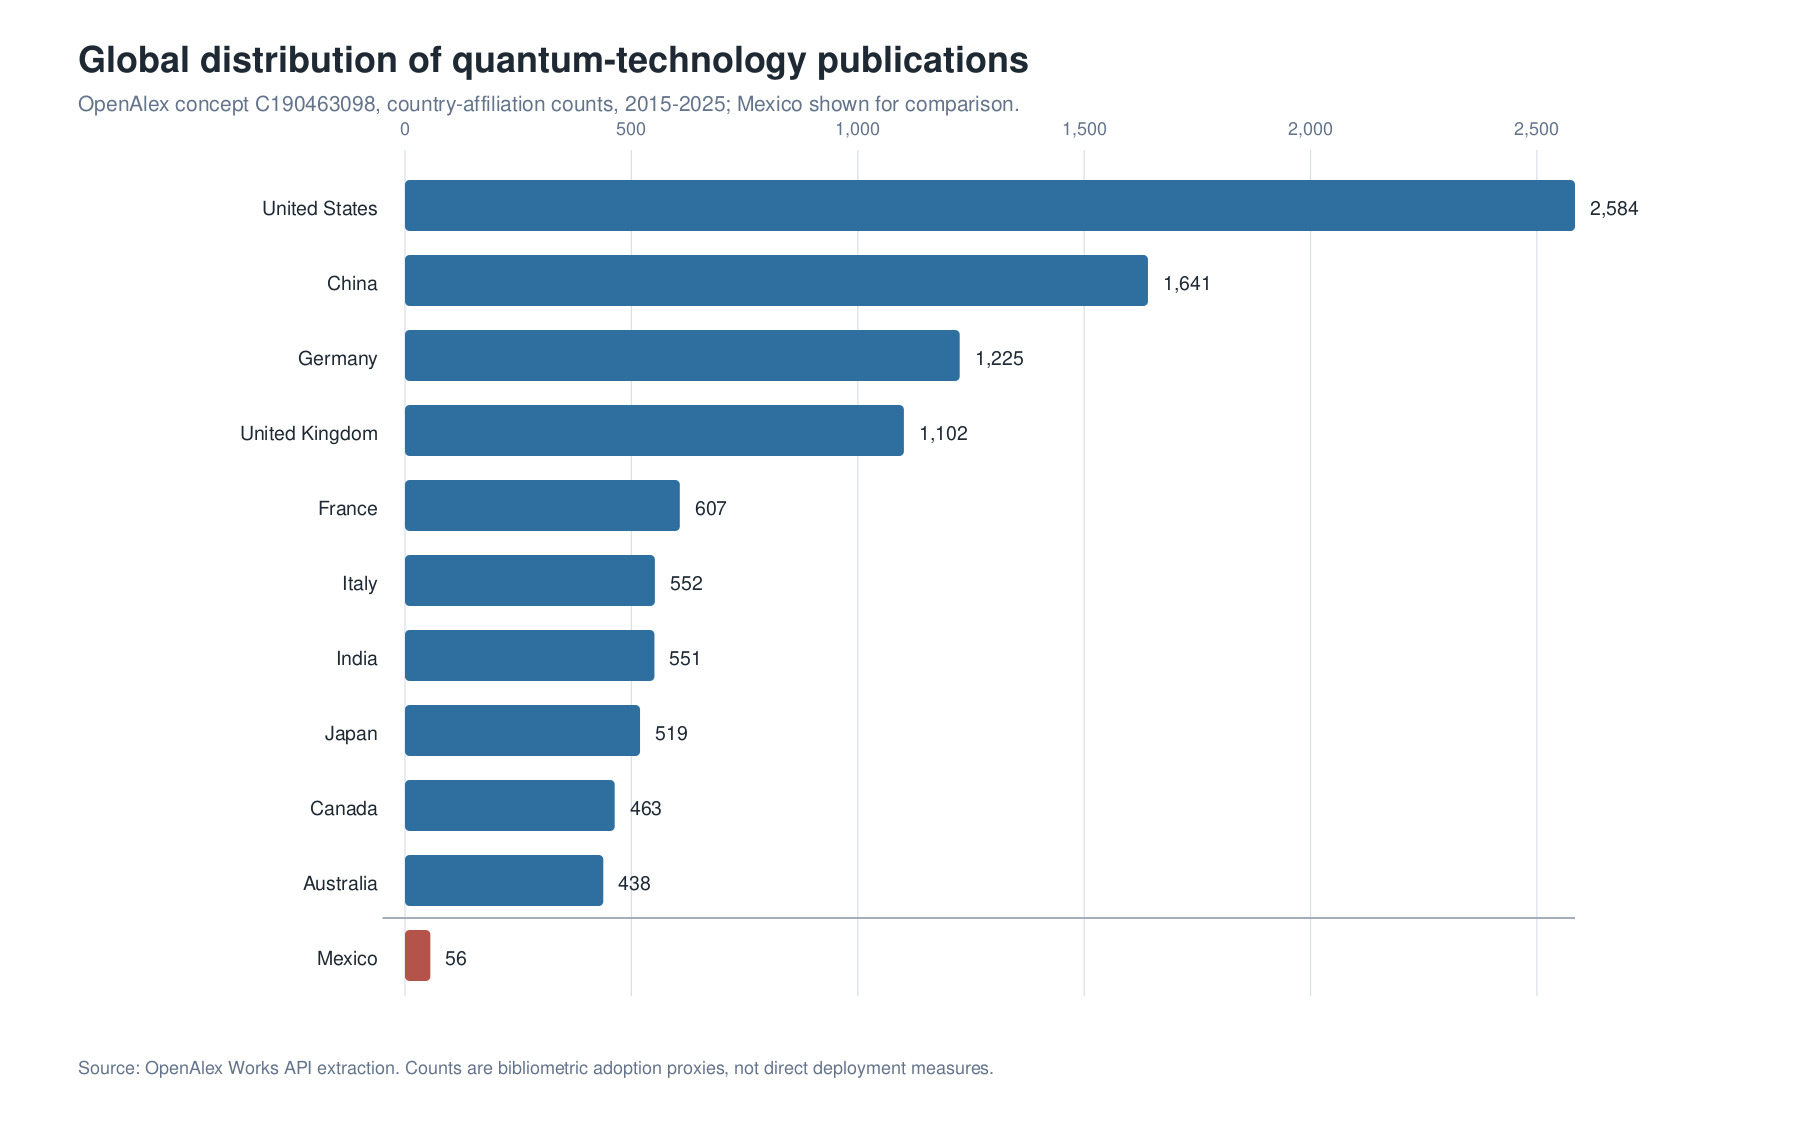
\includegraphics[width=0.95\textwidth,height=\textheight]{figures/fig1_global_country_distribution.png}
\caption{Global distribution of quantum-technology publication capacity.
OpenAlex country-affiliation counts for the concept ``Quantum
technology'' show a concentrated geography led by the United States,
China, Germany, the United Kingdom, and France, with Mexico included as
a comparison case. Counts are bibliometric proxies rather than direct
deployment measures.}
\end{figure}

\begin{figure}
\centering
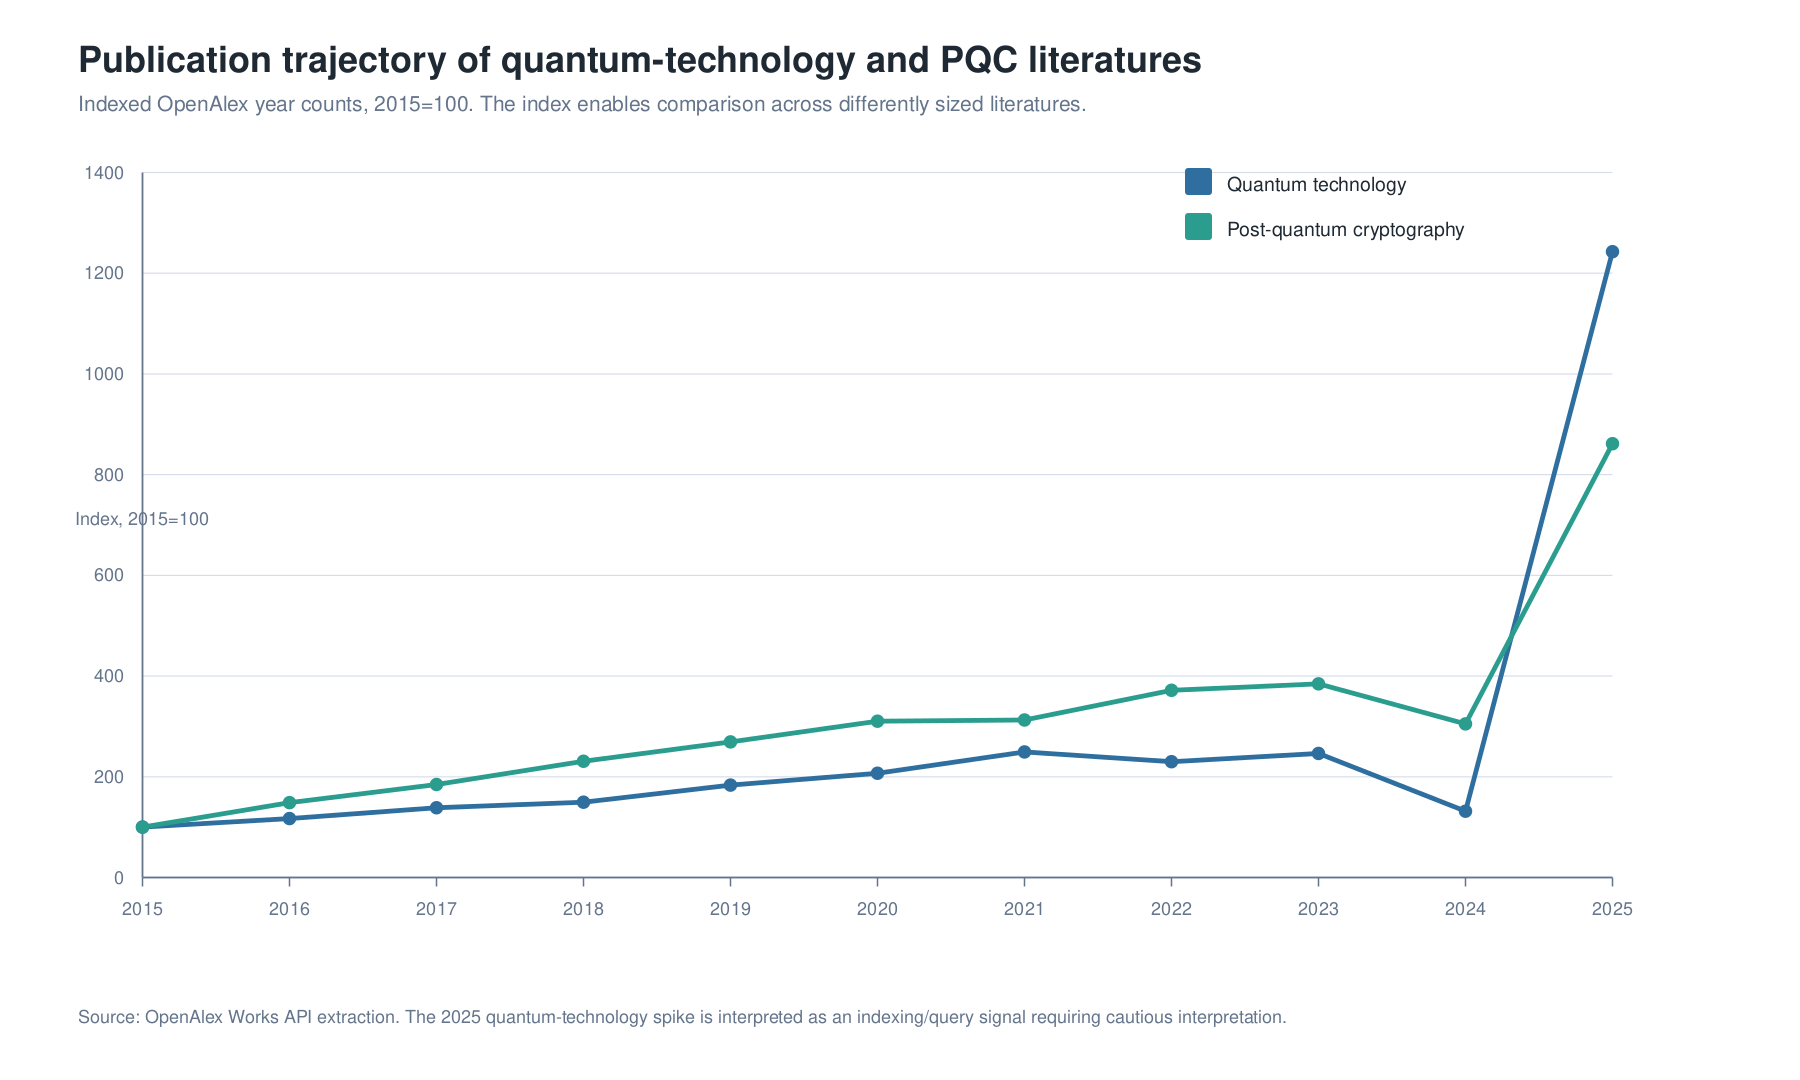
\includegraphics[width=0.95\textwidth,height=\textheight]{figures/fig2_publication_trends.png}
\caption{Indexed publication trajectory for quantum technology and
post-quantum cryptography. OpenAlex annual counts are indexed to
2015=100 to compare differently sized literatures. The 2025
quantum-technology spike is interpreted as a query and indexing signal
requiring cautious interpretation.}
\end{figure}

\section{4. Quantitative Evidence: What Can Be
Measured}\label{quantitative-evidence-what-can-be-measured}

No comprehensive public database currently measures global quantum
adoption directly. There is no single dataset covering deployed quantum
sensors, QKD links, PQC migrations, enterprise pilots, QCaaS usage,
cloud experiments, and quantum software workflows. The evidence is
therefore triangulated across multiple proxies.

\begin{longtable}[]{@{}
  >{\raggedright\arraybackslash}p{(\columnwidth - 4\tabcolsep) * \real{0.3333}}
  >{\raggedright\arraybackslash}p{(\columnwidth - 4\tabcolsep) * \real{0.3333}}
  >{\raggedright\arraybackslash}p{(\columnwidth - 4\tabcolsep) * \real{0.3333}}@{}}
\toprule\noalign{}
\begin{minipage}[b]{\linewidth}\raggedright
Evidence layer
\end{minipage} & \begin{minipage}[b]{\linewidth}\raggedright
Quantitative signal
\end{minipage} & \begin{minipage}[b]{\linewidth}\raggedright
Interpretation
\end{minipage} \\
\midrule\noalign{}
\endhead
\bottomrule\noalign{}
\endlastfoot
Public commitments & OECD reports approximately USD 55.7 billion in
announced public quantum commitments worldwide since 2013, as of October
2025 & Quantum has become a state-level strategic technology \\
Public R\&D awards & OECD Fundstat identifies USD 11.235 billion PPP
across 12,209 quantum-related R\&D awards, 2015-2023 & Public investment
is organized through research and mission programmes \\
Patent families & OECD-EPO mapping identifies 31,700 quantum patent
families with earliest publication years 2005-2024; quantum patenting
increased sevenfold between 2005 and 2024 and grew at about 20 percent
CAGR since 2014 & Invention is accelerating but geographically
concentrated \\
Publications & OpenAlex ``Quantum technology'' query returns 15,279
works, 2015-2025; top countries are the United States, China, Germany,
the United Kingdom, and France & Scientific absorptive capacity is
unevenly distributed \\
PQC publications & OpenAlex PQC query shows the United States, India,
and China as leading country affiliations & PQC readiness depends on
cryptographic and software capacity, not only physics hardware \\
Business readiness & OECD summarizes surveys in which expected
disruption is high but planning, budgets, and use-case identification
are low & Awareness does not equal readiness \\
Standards & NIST finalized ML-KEM, ML-DSA, and SLH-DSA in 2024 & PQC
migration has become an implementation agenda \\
\end{longtable}

The strongest pattern is not simple growth. It is uneven capability
formation. Public funding is rising, patenting is accelerating, and
publications are concentrated in a small set of countries. At the same
time, enterprise readiness remains weak. In the OECD readiness evidence,
97 percent of UK executives in one survey expected quantum disruption,
but only about one-third had begun readiness planning; 87 percent of
financial-sector respondents in another survey viewed quantum as an
opportunity, while 73 percent lacked a commercial-advantage use case and
87 percent lacked a dedicated budget; ISACA evidence summarized by OECD
found that only 20 percent of respondents had formal quantum readiness
plans despite broad expectations of impact (\citeproc{ref-oecd2026}{OECD
2026}).

This is the adoption gap. Countries and firms are hearing the quantum
narrative, but many have not built the mechanisms required to act on it.
The gap is not a public-relations problem. It is a capability problem.

\begin{figure}
\centering
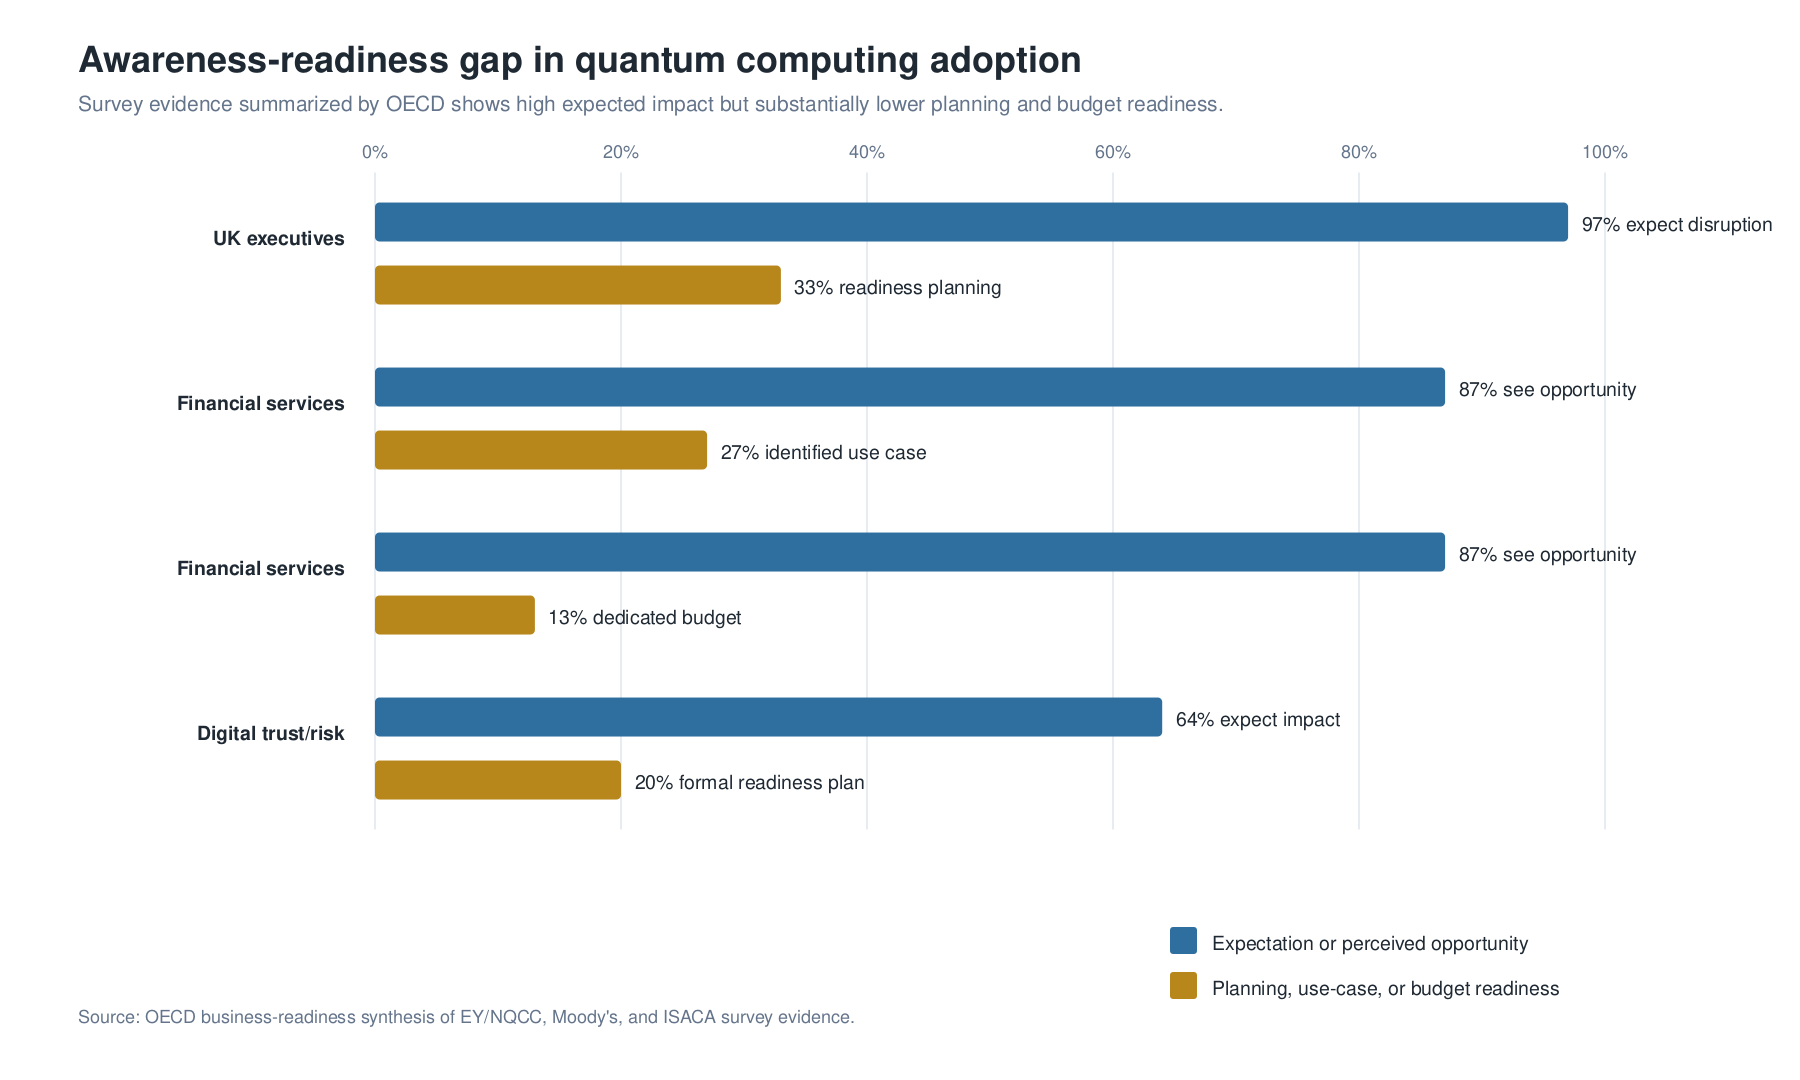
\includegraphics[width=0.95\textwidth,height=\textheight]{figures/fig3_readiness_gap.png}
\caption{Awareness-readiness gap in quantum computing adoption. Survey
evidence summarized by OECD indicates that high expected impact coexists
with substantially lower levels of planning, use-case definition, and
dedicated budget formation.}
\end{figure}

\section{5. Results: Adoption Pathways by Technology
Domain}\label{results-adoption-pathways-by-technology-domain}

\subsection{5.1 Quantum Computing: High Optionality, Low Near-Term
Certainty}\label{quantum-computing-high-optionality-low-near-term-certainty}

Quantum computing has the largest long-term strategic upside and the
greatest adoption uncertainty. Its theoretical foundation is strong.
Quantum algorithms can offer asymptotic speedups in specific problem
classes (\citeproc{ref-montanaro2016}{Montanaro 2016}). Quantum
simulation and chemistry are natural targets because classical computers
struggle with the exponential structure of many quantum systems
(\citeproc{ref-georgescu2014}{Georgescu, Ashhab, and Nori 2014};
\citeproc{ref-cao2019}{Cao et al. 2019}; \citeproc{ref-bauer2020}{Bauer
et al. 2020}). Hybrid variational algorithms offer near-term
experimental pathways (\citeproc{ref-peruzzo2014}{Peruzzo et al. 2014};
\citeproc{ref-kandala2017}{Kandala et al. 2017};
\citeproc{ref-cerezo2021}{Cerezo et al. 2021};
\citeproc{ref-bharti2022}{Bharti et al. 2022}).

The hard constraint is that most valuable applications require deeper
circuits, lower logical error rates, and better verification than
current devices provide. Fault tolerance remains the transition point
from experimental devices to reliable infrastructure. Surface codes
provide a leading approach because they are compatible with
two-dimensional local interactions, but they impose large overheads
(\citeproc{ref-fowler2012}{Fowler et al. 2012};
\citeproc{ref-campbell2017}{Campbell, Terhal, and Vuillot 2017}).
Resource estimates for cryptographically relevant machines remain high,
even when improved algorithms reduce requirements
(\citeproc{ref-gidney2021}{Gidney and Ekera 2021}).

The adoption implication is that quantum computing functions in the near
term as a learning, benchmarking, and option-value domain. The most
rational enterprise and national actions are not mass deployment but
targeted experimentation, workforce formation, algorithmic evaluation,
access to QCaaS platforms, and careful benchmarking against classical
alternatives.

\subsection{5.2 Quantum Sensing: The Most Immediate Public-Value
Domain}\label{quantum-sensing-the-most-immediate-public-value-domain}

Quantum sensing is the strongest near-term application domain because it
can produce value without universal fault-tolerant quantum computers. It
uses quantum systems as measurement devices: atomic clocks for timing,
magnetometers for magnetic fields, gravimeters for subsurface mapping,
inertial sensors for navigation, and quantum defects in diamond for
local magnetic sensing (\citeproc{ref-degen2017}{Degen, Reinhard, and
Cappellaro 2017}; \citeproc{ref-barry2016}{Barry et al. 2016}). The
underlying value proposition is not ``faster computation'' but improved
information about the physical world.

The distinction is important for public policy. Many countries have
urgent problems in water, infrastructure, mining, health, energy,
navigation, border monitoring, seismic risk, environmental monitoring,
and industrial quality control. Quantum sensing can be linked to these
missions earlier than quantum computing can be linked to general
enterprise transformation. The barrier is not theoretical uncertainty
but field deployment: instruments require ruggedization, calibration,
cost-effectiveness, interoperability, and operational relevance.

\subsection{5.3 Quantum Communication: Strategic, Specialized, and
Infrastructure-Heavy}\label{quantum-communication-strategic-specialized-and-infrastructure-heavy}

Quantum communication has strong long-term strategic significance,
especially for entanglement distribution, secure links, distributed
sensing, and future quantum networks (\citeproc{ref-kimble2008}{Kimble
2008}; \citeproc{ref-wehner2018}{Wehner, Elkouss, and Hanson 2018}). QKD
has already moved beyond pure laboratory demonstration, and the security
literature has become sophisticated about realistic devices, side
channels, and measurement-device-independent protocols
(\citeproc{ref-pirandola2020}{Pirandola et al. 2020};
\citeproc{ref-xu2020}{Xu et al. 2020}).

The critique is equally important. QKD does not remove the need for
authentication, endpoint security, network engineering, procurement
standards, or cost-benefit analysis. It requires specialized
infrastructure and can be limited by loss, distance, trusted-node
assumptions, and device assurance. Quantum repeaters are the network
analog of fault tolerance: without reliable repeaters, memories,
entanglement swapping, and low-loss interfaces, large-scale quantum
networks remain constrained.

Consequently, quantum communication is best pursued through targeted
testbeds and high-value links rather than broad claims that it will
replace existing cybersecurity. Its national value lies in strategic
learning, telecom experimentation, high-assurance niches, and
preparation for future quantum networks.

\subsection{5.4 Post-Quantum Cryptography: The First National Adoption
Mandate}\label{post-quantum-cryptography-the-first-national-adoption-mandate}

PQC is the most urgent adoption domain because it addresses a real
security transition that can begin before cryptographically relevant
quantum computers exist. Shor's algorithm threatens RSA, Diffie-Hellman,
and elliptic-curve cryptography once large fault-tolerant machines
exist. The relevant risk is not only future attack; it is present-day
collection of long-lived encrypted data (\citeproc{ref-mosca2018}{Mosca
2018}). NIST's 2024 standards give organizations a concrete migration
target, especially ML-KEM, ML-DSA, and SLH-DSA
(\citeproc{ref-nist2024}{NIST 2024}).

The hard part is not choosing an algorithm in isolation. Migration
requires cryptographic inventories, crypto-agility, vendor coordination,
protocol testing, legacy system replacement, procurement language,
compliance governance, and prioritization by data shelf life. PQC is
therefore a digital-infrastructure programme. Treating it as a narrow
cybersecurity patch underestimates the institutional work involved.

\section{6. Hardware Comparison and Logical-Qubit
Economics}\label{hardware-comparison-and-logical-qubit-economics}

No hardware modality has won. Each platform expresses a different
engineering bargain.

\begin{longtable}[]{@{}
  >{\raggedright\arraybackslash}p{(\columnwidth - 6\tabcolsep) * \real{0.2500}}
  >{\raggedright\arraybackslash}p{(\columnwidth - 6\tabcolsep) * \real{0.2500}}
  >{\raggedright\arraybackslash}p{(\columnwidth - 6\tabcolsep) * \real{0.2500}}
  >{\raggedright\arraybackslash}p{(\columnwidth - 6\tabcolsep) * \real{0.2500}}@{}}
\toprule\noalign{}
\begin{minipage}[b]{\linewidth}\raggedright
Modality
\end{minipage} & \begin{minipage}[b]{\linewidth}\raggedright
Strength
\end{minipage} & \begin{minipage}[b]{\linewidth}\raggedright
Bottleneck
\end{minipage} & \begin{minipage}[b]{\linewidth}\raggedright
Strategic interpretation
\end{minipage} \\
\midrule\noalign{}
\endhead
\bottomrule\noalign{}
\endlastfoot
Superconducting qubits & Fast gates, strong industrial ecosystem,
microfabrication path, cloud availability & Cryogenic wiring, dielectric
loss, crosstalk, thermal load, calibration & Strong near-term platform,
but scale depends on control and error correction economics \\
Trapped ions & High fidelity, long coherence, natural qubit uniformity,
flexible connectivity & Gate speed, shuttling, heating, laser/control
complexity & Excellent quality, but engineering scale and throughput
remain central questions \\
Neutral atoms & Large arrays, reconfigurable geometry, promising
scalability & Atom loss, leakage, gate fidelity, readout, optical
control & Strong option for simulation and scaling, with open questions
about fault-tolerant architecture \\
Photonics & Natural communication medium, room-temperature potential,
networking compatibility & Photon loss, deterministic gates, source and
detector integration & Strategically important for networks and some
computing architectures \\
Quantum annealing & Available systems and optimization experiments &
Limited universality, benchmark ambiguity, mapping overhead & Useful for
experimentation when benchmarked against classical heuristics \\
\end{longtable}

Superconducting platforms have advanced rapidly and are reviewed in
detail by Krantz et al. (\citeproc{ref-krantz2019}{2019}) and Kjaergaard
et al. (\citeproc{ref-kjaergaard2020}{2020}). Trapped-ion systems are
reviewed by Bruzewicz et al. (\citeproc{ref-bruzewicz2019}{2019}).
Neutral atom systems are reviewed by Saffman
(\citeproc{ref-saffman2016}{2016}) and Henriet et al.
(\citeproc{ref-henriet2020}{2020}). Photonic systems are reviewed by
Slussarenko and Pryde (\citeproc{ref-slussarenko2019}{2019}). The
comparison shows why qubit count alone is a weak metric. A device with
more physical qubits may be less valuable than a smaller device with
better gate fidelity, lower correlated noise, better connectivity, or a
clearer route to logical error suppression.

The strategic metric is logical-qubit economics. A useful quantum
computer will not be defined by the number of physical qubits it
contains. It will be defined by the cost, reliability, and speed of
logical operations. Relevant metrics include logical error rate, code
distance, cycle time, decoding latency, leakage, connectivity,
calibration stability, circuit depth at useful fidelity, energy cost,
and physical resources per logical qubit. Proctor et al.
(\citeproc{ref-proctor2022}{2022}) argue that quantum computer
capability is measured by the programmes a processor can run
successfully, not by a single scalar benchmark. This is the standard
required for policy and procurement.

\section{7. Application Domains: Promise, Evidence, and
Critique}\label{application-domains-promise-evidence-and-critique}

\subsection{7.1 Chemistry and Materials}\label{chemistry-and-materials}

Chemistry and materials science remain the strongest long-run
application case. Quantum computers may eventually simulate molecular
and materials systems more naturally than classical machines
(\citeproc{ref-georgescu2014}{Georgescu, Ashhab, and Nori 2014};
\citeproc{ref-cao2019}{Cao et al. 2019}; \citeproc{ref-bauer2020}{Bauer
et al. 2020}). Potential applications include catalysts, batteries,
pharmaceuticals, high-temperature superconductors, corrosion,
fertilizers, polymers, semiconductors, and carbon capture.

The critique is that scientific relevance does not automatically produce
industrial adoption. A useful workflow improves a decision in drug
discovery, materials design, or manufacturing. It produces accuracy that
matters, integrates with laboratory experiments, and reduces time or
cost. The adoption pathway is therefore hybrid: quantum algorithms,
classical high-performance computing, AI models, experiments, and domain
experts working together.

\subsection{7.2 Optimization}\label{optimization}

Optimization is often cited as the earliest commercial opportunity, but
it is also the easiest area to overstate. Logistics, portfolio
optimization, scheduling, grid management, and supply chains are
valuable, but classical optimization is extraordinarily strong.
Mixed-integer programming, constraint programming, heuristics,
approximation algorithms, GPUs, and domain-specific solvers already
perform well. A quantum optimization claim is credible only when it
beats the best classical baseline on a relevant instance at a relevant
cost.

The more realistic near-term role is exploratory: quantum annealing,
QAOA-like workflows, and quantum-inspired methods can help identify
problem classes and software practices. They are not general
replacements for operations research.

\subsection{7.3 Finance}\label{finance}

Finance is attractive because small improvements in risk, optimization,
sampling, or pricing can create large value. Orus, Mugel, and Lizaso
(\citeproc{ref-orus2019}{2019}) and Egger et al.
(\citeproc{ref-egger2020}{2020}) review potential finance applications
including portfolio optimization, Monte Carlo acceleration, risk
analysis, credit scoring, and derivatives pricing. The most serious
institutions will not ask whether quantum computing is fashionable. They
will ask whether it improves model quality, speed, regulatory
auditability, and capital allocation compared with classical methods.

\subsection{7.4 Machine Learning and AI}\label{machine-learning-and-ai}

Quantum machine learning is intellectually rich but commercially
immature. Biamonte et al. (\citeproc{ref-biamonte2017}{2017}) identify
reasons quantum systems may support useful learning models. Schuld and
Killoran (\citeproc{ref-schuld2019}{2019}) connect quantum feature maps
with kernel methods. McClean et al. (\citeproc{ref-mcclean2018}{2018})
show that training can fail through barren plateaus. The resulting
policy advice is straightforward: QML belongs in the research portfolio,
not in exaggerated enterprise transformation claims. The near-term value
may come more from AI improving quantum systems - calibration, error
mitigation, pulse design, materials discovery, and control - than from
quantum systems improving mainstream AI.

\subsection{7.5 Cybersecurity}\label{cybersecurity}

Cybersecurity is the most immediate cross-sectoral application because
PQC migration affects almost every digital system. The core policy issue
is time. Data requiring confidentiality for 10, 20, or 30 years may be
vulnerable to future quantum decryption. Large organizations may need
many years to inventory and migrate cryptographic assets. If the sum of
data shelf life and migration time exceeds the time to a
cryptographically relevant quantum computer, action is late by
definition (\citeproc{ref-mosca2018}{Mosca 2018}).

\section{8. High-Performance Computing and Quantum
Computing}\label{high-performance-computing-and-quantum-computing}

The adoption pathway for quantum computing is inseparable from
high-performance computing. Quantum computers are unlikely to replace
classical supercomputers as general-purpose machines. The more plausible
transition is an accelerator model in which quantum processing units are
integrated into heterogeneous HPC environments alongside CPUs, GPUs,
storage systems, workflow managers, schedulers, and scientific software
stacks. In this architecture, quantum computation is invoked only for
subroutines where a quantum representation may improve simulation,
sampling, optimization, or linear-algebra tasks, while classical HPC
performs data preparation, orchestration, error mitigation, optimization
loops, verification, and post-processing.

Recent HPC-QC research reflects this transition. Cranganore et al.
(\citeproc{ref-cranganore2024}{2024}) formalize hybrid quantum-classical
scientific workflows and identify workflow-management requirements for
mapping classical scientific pipelines onto hybrid resources. Beck et
al. (\citeproc{ref-beck2024}{2024}) frame quantum computing as a
computational accelerator within scientific HPC ecosystems, emphasizing
hardware-agnostic integration, benchmarks, user interfaces, and workflow
management. Liu et al. (\citeproc{ref-liu2024}{2024}) develop a
quantum-centric HPC perspective for quantum chemistry, where quantum
algorithms, quantum emulators, and classical HPC resources jointly
support chemical simulation. This literature shifts the question from
``when will quantum computers replace supercomputers?'' to ``which
components of a scientific workflow can be delegated to a QPU under
realistic latency, noise, queueing, and verification constraints?''

The HPC view changes four elements of quantum strategy. First, it
changes infrastructure. A useful quantum computing ecosystem requires
not only QPUs and cloud accounts, but also schedulers, middleware,
compilers, error-mitigation software, data movement protocols,
provenance systems, reproducibility controls, and interfaces with
existing scientific codes. Second, it changes benchmarking. A quantum
subroutine must be evaluated inside a full workflow, including
data-loading cost, classical optimization time, queue latency,
error-mitigation overhead, and validation against classical HPC
baselines. Third, it changes workforce formation. Quantum computing
adoption requires computational scientists and HPC engineers who can
decompose applications into classical and quantum components, not only
physicists who understand qubits. Fourth, it changes national
procurement. A country that invests in quantum computing without HPC
integration capacity risks buying isolated devices that cannot support
scientific or industrial workflows.

The complementarity is especially important for middle-income and
emerging quantum economies. Domestic ownership of a leading quantum
computer may be unrealistic in the short run, but access to HPC centers,
GPU clusters, scientific workflow systems, and cloud-based QPUs can
still create meaningful absorptive capacity. The strategic objective is
therefore not a binary transition from HPC to quantum computing. It is
the construction of an HPC-QC continuum in which classical
supercomputing remains the operational substrate and quantum computing
enters as a specialized accelerator when evidence justifies it.

\section{9. Comparative National
Strategy}\label{comparative-national-strategy}

Different national models reveal different strategic theories.

The United States combines federal coordination, national laboratories,
universities, venture capital, major cloud platforms, and defense-linked
research. Its advantage is ecosystem diversity and private capital
depth. Its weakness is fragmentation and uneven translation across
agencies and sectors.

China has emphasized state-directed investment, secure communication
infrastructure, and technological self-reliance. Its advantage is
coordination and strategic focus. Its weakness may be lower transparency
and a risk of overbuilding symbolic infrastructure before operational
value is clear.

Europe emphasizes cross-border coordination, public research networks,
standards, and strategic autonomy. Its advantage is institutional
coordination and research quality. Its weakness is commercialization
speed and fragmentation across national markets.

Middle-income and manufacturing-intensive countries face a different
problem. They cannot simply copy the largest programmes. Their strategic
opportunity is selective capability building: PQC migration, quantum
sensing for public missions, cloud-mediated access to quantum computing,
metrology laboratories, workforce networks, and participation in
standards. The right goal is not to immediately own every layer of the
stack. It is to avoid becoming merely a buyer of quantum technologies
designed, benchmarked, and governed elsewhere.

\section{10. Toward a National Quantum Capability
Model}\label{toward-a-national-quantum-capability-model}

The evidence supports a capability model with seven pillars.

\begin{longtable}[]{@{}
  >{\raggedright\arraybackslash}p{(\columnwidth - 4\tabcolsep) * \real{0.3333}}
  >{\raggedright\arraybackslash}p{(\columnwidth - 4\tabcolsep) * \real{0.3333}}
  >{\raggedright\arraybackslash}p{(\columnwidth - 4\tabcolsep) * \real{0.3333}}@{}}
\toprule\noalign{}
\begin{minipage}[b]{\linewidth}\raggedright
Pillar
\end{minipage} & \begin{minipage}[b]{\linewidth}\raggedright
Core capability
\end{minipage} & \begin{minipage}[b]{\linewidth}\raggedright
Main institutional question
\end{minipage} \\
\midrule\noalign{}
\endhead
\bottomrule\noalign{}
\endlastfoot
Scientific frontier & Research in quantum information, algorithms,
metrology, materials, error correction, foundations & Can the country
participate in frontier knowledge production? \\
Security transition & PQC migration, crypto-agility, long-lived data
protection & Can critical systems remain secure through the quantum
transition? \\
Sensing and metrology & Atomic clocks, magnetometry, gravimetry,
inertial sensing, calibration & Can quantum measurement solve national
problems in territory, water, health, energy, and infrastructure? \\
HPC-QC computing access & QCaaS, HPC integration, hybrid workflows,
benchmarks, quantum software & Can institutions learn without premature
hardware lock-in while preserving continuity with scientific computing
infrastructure? \\
Standards and procurement & Benchmarking, interoperability, vendor
evaluation, anti-hype criteria & Can public and private buyers
distinguish performance from narrative? \\
Workforce & Researchers, engineers, technicians, cybersecurity
professionals, procurement officers & Can the ecosystem build the
missing middle between physics PhDs and operational deployment? \\
Industrial position & Components, control systems, photonics,
cryogenics, software, sensing integration & Where can domestic firms
enter the value chain realistically? \\
\end{longtable}

The workforce pillar deserves emphasis. Kaur and Venegas-Gomez
(\citeproc{ref-kaur2022}{2022}) show that quantum education initiatives
are expanding globally, but the workforce problem is not only a need for
more PhDs. Quantum industries require technicians and engineers who can
align lasers, operate cryostats, build RF control systems, manage vacuum
systems, write firmware, perform calibration, design software
interfaces, audit cryptography, and translate domain problems into
testable workflows. A nation that trains only researchers but not
operators will remain dependent on imported systems.

\begin{figure}
\centering
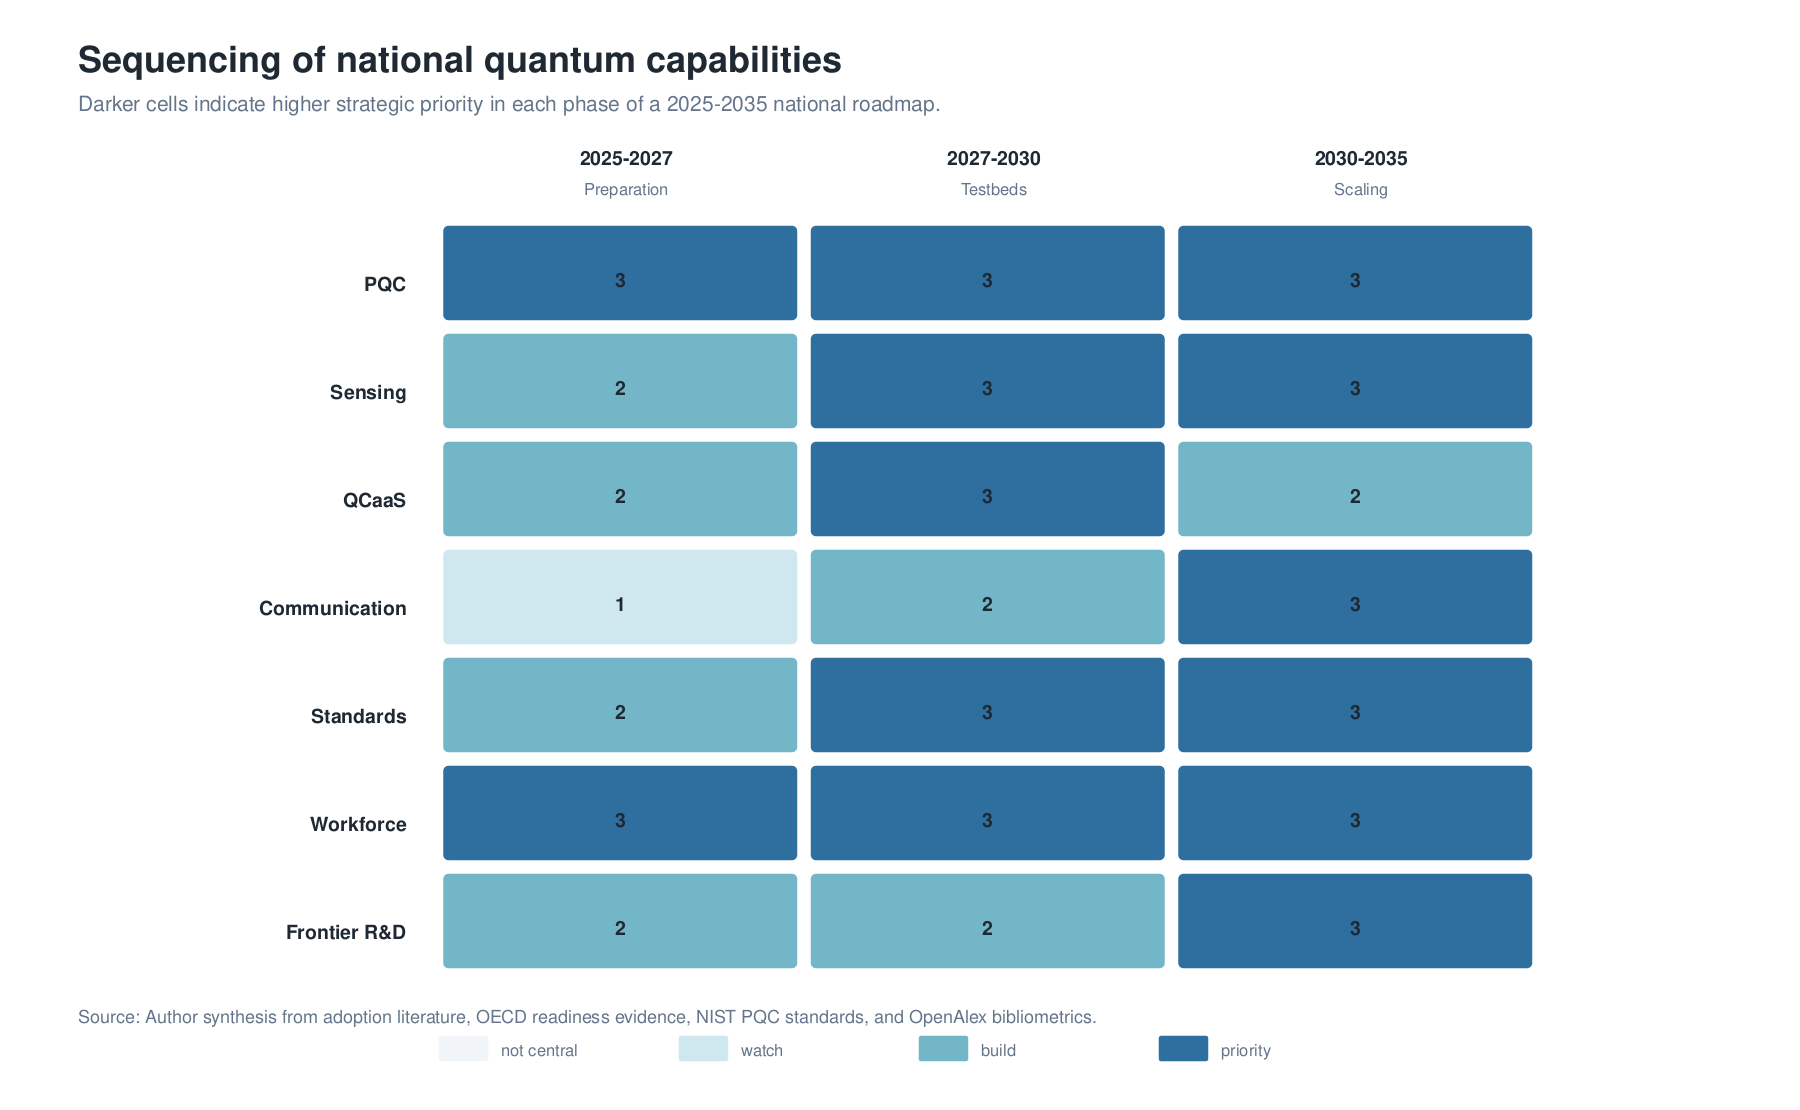
\includegraphics[width=0.95\textwidth,height=\textheight]{figures/fig4_capability_heatmap.png}
\caption{Sequencing of national quantum capabilities. The heatmap scores
strategic priority across three roadmap phases, emphasizing that PQC,
workforce, standards, sensing, QCaaS, communication, and frontier R\&D
mature on different policy timelines.}
\end{figure}

\section{11. Strategic Roadmap,
2025-2035}\label{strategic-roadmap-2025-2035}

\subsection{11.1 Phase I: Preparation and Security,
2025-2027}\label{phase-i-preparation-and-security-2025-2027}

The first phase is not about buying a national quantum computer. It is
about becoming a competent adopter. Core institutional actions include a
quantum readiness office, cryptographic asset inventories, PQC migration
priorities for long-lived data, procurement language for quantum-safe
systems, quantum sensing feasibility studies, QCaaS access for
universities and agencies, HPC-QC workflow training, and workforce
modules for engineers, cybersecurity professionals, and public-sector
decision makers.

The measurable outputs are not press releases. They are inventories,
trained personnel, use-case pipelines, testable requirements,
procurement standards, and baseline institutional competence.

\subsection{11.2 Phase II: Testbeds and Mission Pilots,
2027-2030}\label{phase-ii-testbeds-and-mission-pilots-2027-2030}

The second phase centers on operational learning. Quantum sensing pilots
can be linked to water, energy, health, geodesy, infrastructure, mining,
and environmental risk. PQC migration moves from planning to staged
implementation. Quantum software testbeds evaluate algorithms against
classical baselines. HPC centers test hybrid quantum-classical
workflows, including scheduler integration, simulator-to-hardware
transition, and workflow provenance. Telecom and research institutions
can test QKD and early network components where high-value links justify
the cost. Standards laboratories evaluate vendor claims.

The main risk in this phase is quantum washing. Vendors and agencies may
label classical, quantum-inspired, or immature systems as strategic
breakthroughs. The protection is benchmark discipline: every pilot
requires a classical baseline, a performance metric, a cost metric, a
verification method, and a decision rule.

\subsection{11.3 Phase III: Selective Scaling and Frontier Integration,
2030-2035}\label{phase-iii-selective-scaling-and-frontier-integration-2030-2035}

The third phase scales only what has demonstrated value. Sensing systems
that solve mission problems can move into procurement. PQC can become
standard across public digital infrastructure. Quantum computing can
expand where workflows show credible advantage or where workforce and
scientific value justify continued experimentation. National research
deepens in error correction, logical qubits, quantum repeaters,
device-independent security, quantum metrology, quantum materials, and
foundations.

\begin{figure}
\centering
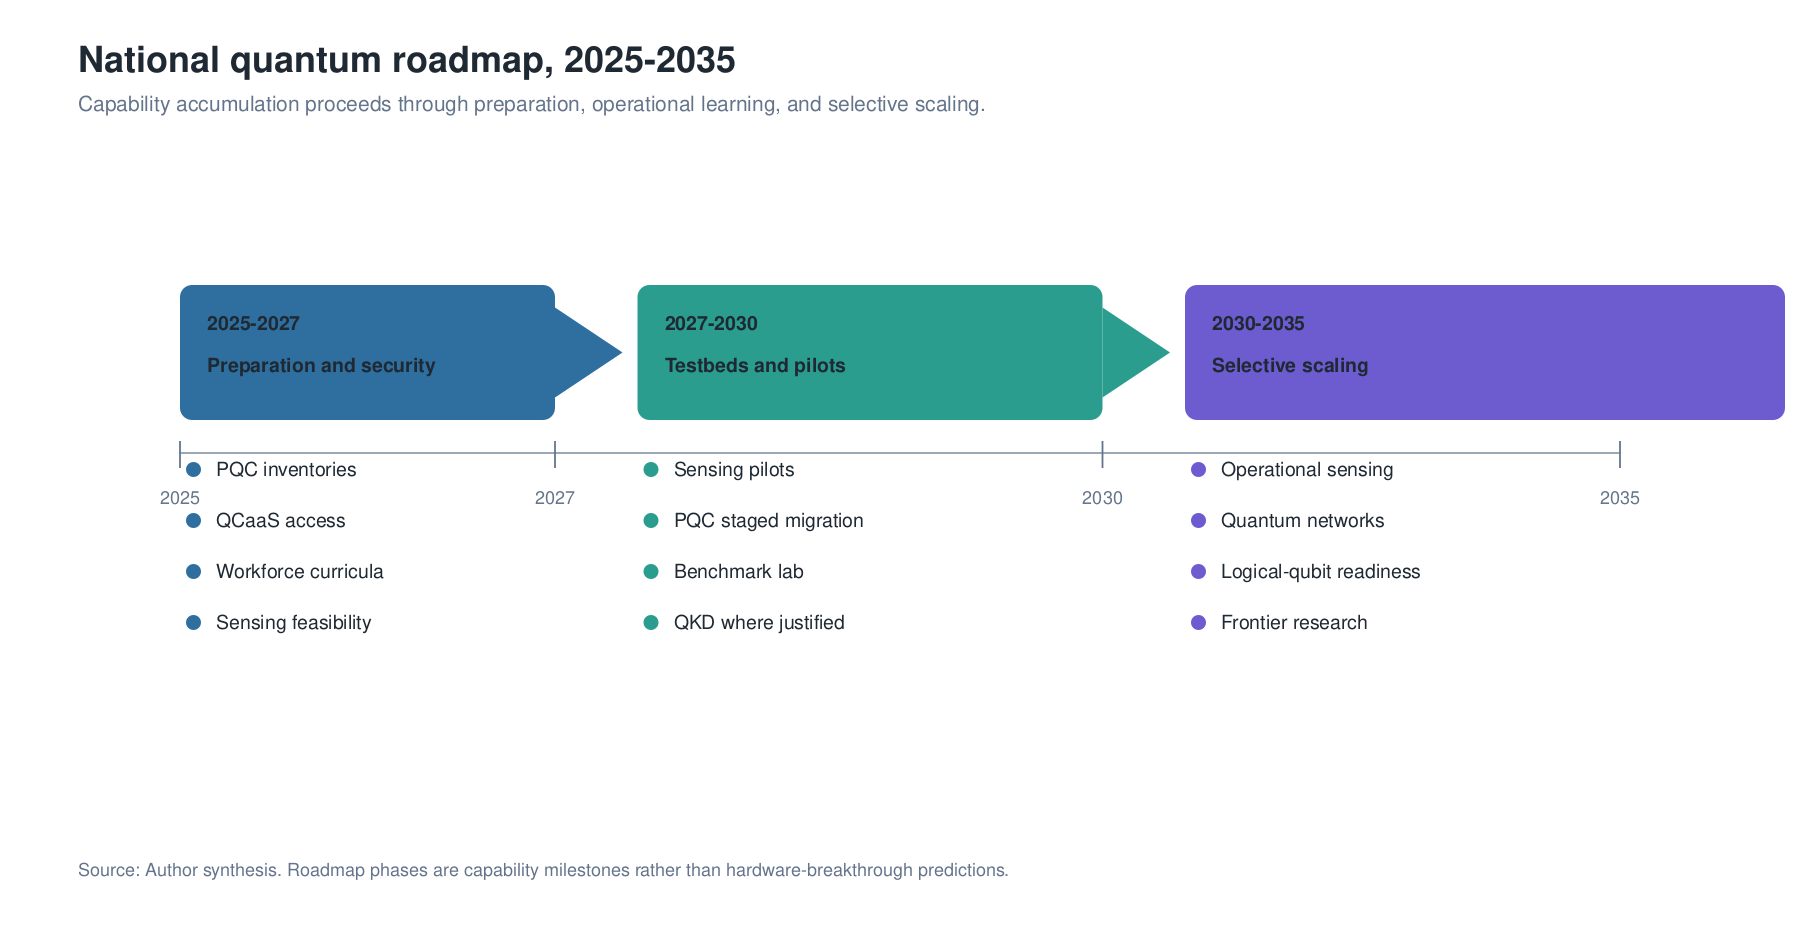
\includegraphics[width=0.95\textwidth,height=\textheight]{figures/fig5_roadmap_timeline.png}
\caption{Roadmap for national quantum capability formation, 2025-2035.
The sequence is organized around institutional readiness, operational
learning, and selective scaling rather than prediction of a single
hardware breakthrough.}
\end{figure}

The strategic objective is optionality. By 2035, the successful nation
is not necessarily the one with the largest announced quantum computer.
It is the one with trained people, secure cryptography, functioning
testbeds, standards capacity, metrology capability, domain pilots,
international partnerships, and a research base connected to the
frontier.

\section{12. Frontier Research Agenda}\label{frontier-research-agenda}

National quantum strategy includes frontier topics that are not
immediately commercial. These areas generate instruments, expertise, and
long-term autonomy.

\textbf{Logical-qubit economics.} Research moves from physical qubit
counts to logical operation cost. This includes error correction,
decoders, leakage management, magic-state overhead, qLDPC codes, and
architecture-specific resource estimates.

\textbf{Quantum network break-even.} Quantum repeaters, memories,
transducers, and entanglement swapping are the network equivalent of
fault tolerance. The milestone is not a laboratory link alone; it is
performance beyond direct transmission under realistic cost and
reliability constraints.

\textbf{Quantum sensing for national missions.} Research connects
gravimetry, magnetometry, timing, and inertial sensing to real public
problems. The central question is not maximum sensitivity in isolation,
but operational value under field conditions.

\textbf{Benchmark science.} Nations need independent capability to test
quantum claims. This includes randomized benchmarking, application-level
benchmarks, error characterization, reproducibility, and cost-based
performance metrics (\citeproc{ref-proctor2022}{Proctor et al. 2022};
\citeproc{ref-alexeev2021}{Alexeev et al. 2021}).

\textbf{Quantum foundations as instrumentation strategy.} Foundational
work on contextuality, measurement, macroscopic superposition,
decoherence, and non-Markovian noise is not merely philosophical. It
drives instrumentation in interferometry, isolation, optics, cryogenics,
detectors, and control.

\textbf{AI for quantum systems.} AI may be most valuable as a tool for
quantum engineering: calibration, control, error mitigation, materials
discovery, scheduling, pulse optimization, and interpretation of sensor
data.

\section{13. Discussion: What a Serious Quantum Strategy Must
Avoid}\label{discussion-what-a-serious-quantum-strategy-must-avoid}

The first error is waiting. Waiting for fault-tolerant machines before
preparing for PQC, workforce, standards, and sensing would leave
institutions unprepared when adoption pressure rises. Readiness takes
years.

The second error is hardware nationalism without capability. Buying or
announcing a domestic quantum computer does not create a quantum
ecosystem if there are no trained operators, no benchmarking laboratory,
no software pipeline, no procurement discipline, and no mission demand.

The third error is confusing QKD with PQC. QKD may be valuable for
specialized links and research networks, but PQC is the broad migration
path for existing digital systems. Treating QKD as a general substitute
for PQC misreads both the technology and the infrastructure problem.

The fourth error is treating QCaaS as neutral access. Cloud access
democratizes experimentation, but it can also concentrate platform
power. The cloud provider may control developer tools, backend access,
pricing, data policies, and enterprise relationships. Nations need QCaaS
access, but they also need sovereignty over knowledge, benchmarks,
critical data governance, and the ability to connect quantum experiments
to domestic HPC infrastructure.

The fifth error is accepting quantum advantage claims without baselines.
A credible claim specifies the problem class, classical baseline,
hardware assumptions, error model, verification method,
time-to-solution, energy cost, and economic relevance. Without these
elements, the claim is not a procurement basis.

The sixth error is underfunding the missing middle. Quantum strategy
often funds elite research and startup promotion while ignoring
technicians, engineers, standards experts, cybersecurity auditors, and
procurement professionals. These roles determine whether science becomes
infrastructure.

\section{14. Policy and Enterprise
Recommendations}\label{policy-and-enterprise-recommendations}

For national governments, the first recommendation is to create a
quantum readiness function with authority across science, economy,
cybersecurity, defense, education, standards, and public procurement.
Fragmented committees are insufficient if they cannot set priorities or
coordinate budgets.

Second, PQC migration is critical digital infrastructure. The correct
unit of work is not only algorithm selection. It is asset inventory,
data-shelf-life classification, crypto-agility, vendor management,
testing, staged migration, and compliance.

Third, quantum sensing is best funded through mission pilots. Water,
energy, health, territory, infrastructure, mining, navigation, and
environmental monitoring offer public-value use cases where better
measurement can change decisions.

Fourth, quantum computing policy emphasizes HPC integration, access,
benchmarks, and talent before domestic hardware lock-in. QCaaS, shared
testbeds, open software, and hybrid workflow managers can build
competence while hardware trajectories remain uncertain.

Fifth, public procurement requires anti-hype evidence. Every quantum
pilot includes a classical baseline, performance metric, cost metric,
interoperability requirement, security assessment, and exit criterion.

Sixth, the research system funds frontier science and industrialization
together. Error correction, repeaters, metrology, foundations,
materials, and control systems are not separate from commercialization;
they are the base from which commercialization will emerge.

For enterprises, the first step is not a large quantum transformation
programme. It is a small readiness portfolio: identify high-value
problems, map cryptographic risk, train technical staff, test QCaaS
workflows, track standards, and join consortia. Investment is justified
when a quantum method improves a decision, not when it improves a
narrative.

\section{15. Conclusion}\label{conclusion}

Quantum technologies will shape the next decade less through sudden
universal disruption than through uneven capability formation. PQC is
already a cybersecurity migration problem. Quantum sensing can produce
public and industrial value before fault-tolerant computing. Quantum
communication is strategically important but infrastructure-heavy.
Quantum computing remains the largest long-term opportunity, but its
value depends on logical-qubit economics, verified advantage, and
integration with classical workflows.

The most important conclusion is that quantum readiness is a national
capability, not a hardware purchase. Countries that build cryptographic
migration capacity, sensing pilots, standards laboratories, workforce
pathways, QCaaS competence, and frontier research networks will be
positioned to adopt whichever hardware modalities mature. Countries that
wait for the market to deliver finished quantum products will become
dependent buyers.

The future of quantum technologies therefore requires disciplined
ambition. The ambition is to build scientific and technological
sovereignty in a field that will affect security, measurement,
computation, and industrial discovery. The discipline is evidentiary:
rigorous science, reproducible benchmarks, classical baselines,
operational pilots, and transparent procurement. Quantum strategy
succeeds when it turns fragile quantum effects into reliable public
capability.

\section{Acknowledgments}\label{acknowledgments}

This manuscript was prepared for the Quantum Technologies track of the
twenty-third edition of the Global Information Technology Management
Association Annual Conference, Monterrey, Mexico, May 6-8, 2026. The
author acknowledges his role as Track Chair for Quantum Technologies and
gratefully acknowledges Rogelio Marín and the Centro de Investigación en
Matemáticas, A.C. for intellectual support and institutional context.
All interpretations and remaining errors are the author's
responsibility.

\section{Data Availability}\label{data-availability}

The quantitative tables generated for this manuscript are deposited in
the companion research repository. They include OpenAlex country and
year counts for the concepts ``Quantum technology'' and ``Post-quantum
cryptography'' for 2015-2025. OECD, NIST, NSA, CISA, OECD-EPO, and
market-readiness data are cited to public sources in the reference list.
The OpenAlex queries used concept IDs \texttt{C190463098} and
\texttt{C108277079}, grouped by publication year and institutional
country.

\section{Code Availability}\label{code-availability}

The companion research repository is available at
https://github.com/ekaropolus/quantum-technologies-national-strategy. It
contains the source manuscripts, processed data, BibTeX bibliography,
figure-generation code, and reproducible build script used to generate
the manuscript outputs. The repository is intended to support inspection
of the OpenAlex extracts, regeneration of figures, and reconstruction of
the PDF, TeX, and DOCX versions from the manuscript sources.

\section{Author Contributions}\label{author-contributions}

Edgar Valdés conceptualized the manuscript, directed the research
synthesis, interpreted the evidence, and prepared the manuscript.

\section{Funding}\label{funding}

No external funding was declared for this manuscript.

\section{Competing Interests}\label{competing-interests}

The author declares no competing interests.

\section{Limitations}\label{limitations}

The analysis relies on adoption proxies rather than direct global
deployment data. Funding, patents, publications, standards, and
readiness surveys measure different dimensions of quantum capacity and
are not interchangeable. OpenAlex counts depend on concept assignment,
institutional metadata, and indexing practices. Market forecasts are
treated only as directional evidence. A future empirical extension would
require interviews with government agencies, infrastructure operators,
quantum vendors, cybersecurity teams, and enterprise adopters, plus a
structured survey of quantum readiness across sectors.

\section{References}\label{references}

\phantomsection\label{refs}
\begin{CSLReferences}{1}{0}
\bibitem[\citeproctext]{ref-acin2018}
Acin, Antonio, Immanuel Bloch, Harry Buhrman, Tommaso Calarco,
Christopher Eichler, Jens Eisert, Daniel Esteve, et al. 2018. {``The
Quantum Technologies Roadmap: A European Community View.''} \emph{New
Journal of Physics} 20: 080201.
\url{https://doi.org/10.1088/1367-2630/aad1ea}.

\bibitem[\citeproctext]{ref-alexeev2021}
Alexeev, Yuri, Dave Bacon, Kenneth R. Brown, Robert Calderbank, Lincoln
D. Carr, Frederic T. Chong, Brian DeMarco, et al. 2021. {``Quantum
Computer Systems for Scientific Discovery.''} \emph{PRX Quantum} 2:
017001. \url{https://doi.org/10.1103/PRXQuantum.2.017001}.

\bibitem[\citeproctext]{ref-arute2019}
Arute, Frank, Kunal Arya, Ryan Babbush, Dave Bacon, Joseph C. Bardin,
Rami Barends, Rupak Biswas, et al. 2019. {``Quantum Supremacy Using a
Programmable Superconducting Processor.''} \emph{Nature} 574: 505--10.
\url{https://doi.org/10.1038/s41586-019-1666-5}.

\bibitem[\citeproctext]{ref-barry2016}
Barry, John F., Matthew J. Turner, Jennifer M. Schloss, David R. Glenn,
Yuyu Song, Mikhail D. Lukin, Hongkun Park, and Ronald L. Walsworth.
2016. {``Optical Magnetic Detection of Single-Neuron Action Potentials
Using Quantum Defects in Diamond.''} \emph{Proceedings of the National
Academy of Sciences} 113 (49): 14133--38.
\url{https://doi.org/10.1073/pnas.1601513113}.

\bibitem[\citeproctext]{ref-bauer2020}
Bauer, Bela, Sergey Bravyi, Mario Motta, and Garnet Kin-Lic Chan. 2020.
{``Quantum Algorithms for Quantum Chemistry and Quantum Materials
Science.''} \emph{Chemical Reviews} 120 (22): 12685--717.
\url{https://doi.org/10.1021/acs.chemrev.9b00829}.

\bibitem[\citeproctext]{ref-beck2024}
Beck, Thomas, Alessandro Baroni, Ryan Bennink, Gilles Buchs, Eduardo
Antonio Coello Perez, Markus Eisenbach, Rafael Ferreira da Silva, et al.
2024. {``Integrating Quantum Computing Resources into Scientific HPC
Ecosystems.''} \emph{Future Generation Computer Systems}.
\url{https://doi.org/10.1016/j.future.2024.06.058}.

\bibitem[\citeproctext]{ref-bernstein2017}
Bernstein, Daniel J., and Tanja Lange. 2017. {``Post-Quantum
Cryptography.''} \emph{Nature} 549: 188--94.
\url{https://doi.org/10.1038/nature23461}.

\bibitem[\citeproctext]{ref-bharti2022}
Bharti, Kishor, Alba Cervera-Lierta, Thi Ha Kyaw, Tobias Haug, Sumner
Alperin-Lea, Abhinav Anand, Matthias Degroote, et al. 2022. {``Noisy
Intermediate-Scale Quantum Algorithms.''} \emph{Reviews of Modern
Physics} 94: 015004. \url{https://doi.org/10.1103/RevModPhys.94.015004}.

\bibitem[\citeproctext]{ref-biamonte2017}
Biamonte, Jacob, Peter Wittek, Nicola Pancotti, Patrick Rebentrost,
Nathan Wiebe, and Seth Lloyd. 2017. {``Quantum Machine Learning.''}
\emph{Nature} 549: 195--202. \url{https://doi.org/10.1038/nature23474}.

\bibitem[\citeproctext]{ref-bova2020}
Bova, Francesco, Avi Goldfarb, and Roger G. Melko. 2020. {``The Emerging
Commercial Landscape of Quantum Computing.''} \emph{Nature Reviews
Physics} 2: 596--98. \url{https://doi.org/10.1038/s42254-020-00247-5}.

\bibitem[\citeproctext]{ref-bruzewicz2019}
Bruzewicz, Colin D., John Chiaverini, Robert McConnell, and Jeremy M.
Sage. 2019. {``Trapped-Ion Quantum Computing: Progress and
Challenges.''} \emph{Applied Physics Reviews} 6: 021314.
\url{https://doi.org/10.1063/1.5088164}.

\bibitem[\citeproctext]{ref-campbell2017}
Campbell, Earl T., Barbara M. Terhal, and Christophe Vuillot. 2017.
{``Roads Towards Fault-Tolerant Universal Quantum Computation.''}
\emph{Nature} 549: 172--79. \url{https://doi.org/10.1038/nature23460}.

\bibitem[\citeproctext]{ref-cao2019}
Cao, Yudong, Jonathan Romero, Jonathan P. Olson, Matthias Degroote,
Peter D. Johnson, Maria Kieferova, Ian D. Kivlichan, et al. 2019.
{``Quantum Chemistry in the Age of Quantum Computing.''} \emph{Chemical
Reviews} 119 (19): 10856--915.
\url{https://doi.org/10.1021/acs.chemrev.8b00803}.

\bibitem[\citeproctext]{ref-cerezo2021}
Cerezo, Marco, Andrew Arrasmith, Ryan Babbush, Simon C. Benjamin, Suguru
Endo, Keisuke Fujii, Jarrod R. McClean, et al. 2021. {``Variational
Quantum Algorithms.''} \emph{Nature Reviews Physics} 3: 625--44.
\url{https://doi.org/10.1038/s42254-021-00348-9}.

\bibitem[\citeproctext]{ref-cisaNistNsa2022}
CISA, NIST, and NSA. 2022. {``Preparing Critical Infrastructure for
Post-Quantum Cryptography.''}
\url{https://www.cisa.gov/sites/default/files/2022-09/cisa_insight_post_quantum_cryptography_508.pdf}.

\bibitem[\citeproctext]{ref-cohen1990}
Cohen, Wesley M., and Daniel A. Levinthal. 1990. {``Absorptive Capacity:
A New Perspective on Learning and Innovation.''} \emph{Administrative
Science Quarterly} 35 (1): 128--52.
\url{https://doi.org/10.2307/2393553}.

\bibitem[\citeproctext]{ref-cranganore2024}
Cranganore, Sandeep Suresh, Vincenzo De Maio, Ivona Brandic, and Ewa
Deelman. 2024. {``Paving the Way to Hybrid Quantum-Classical Scientific
Workflows.''} \emph{Future Generation Computer Systems} 158: 346--66.
\url{https://doi.org/10.1016/j.future.2024.04.030}.

\bibitem[\citeproctext]{ref-degen2017}
Degen, C. L., F. Reinhard, and P. Cappellaro. 2017. {``Quantum
Sensing.''} \emph{Reviews of Modern Physics} 89: 035002.
\url{https://doi.org/10.1103/RevModPhys.89.035002}.

\bibitem[\citeproctext]{ref-dowling2003}
Dowling, Jonathan P., and Gerard J. Milburn. 2003. {``Quantum
Technology: The Second Quantum Revolution.''} \emph{Philosophical
Transactions of the Royal Society A} 361 (1809): 1655--74.
\url{https://doi.org/10.1098/rsta.2003.1227}.

\bibitem[\citeproctext]{ref-egger2020}
Egger, Daniel J., Claudio Gambella, Jakub Marecek, Scott McFaddin,
Martin Mevissen, Rudy Raymond, Andrea Simonetto, Stefan Woerner, and
Elena Yndurain. 2020. {``Quantum Computing for Finance: State-of-the-Art
and Future Prospects.''} \emph{IEEE Transactions on Quantum Engineering}
1: 1--24. \url{https://doi.org/10.1109/TQE.2020.3030314}.

\bibitem[\citeproctext]{ref-fowler2012}
Fowler, Austin G., Matteo Mariantoni, John M. Martinis, and Andrew N.
Cleland. 2012. {``Surface Codes: Towards Practical Large-Scale Quantum
Computation.''} \emph{Physical Review A} 86: 032324.
\url{https://doi.org/10.1103/PhysRevA.86.032324}.

\bibitem[\citeproctext]{ref-georgescu2014}
Georgescu, I. M., S. Ashhab, and Franco Nori. 2014. {``Quantum
Simulation.''} \emph{Reviews of Modern Physics} 86: 153--85.
\url{https://doi.org/10.1103/RevModPhys.86.153}.

\bibitem[\citeproctext]{ref-gidney2021}
Gidney, Craig, and Martin Ekera. 2021. {``How to Factor 2048 Bit RSA
Integers in 8 Hours Using 20 Million Noisy Qubits.''} \emph{Quantum} 5:
433. \url{https://doi.org/10.22331/q-2021-04-15-433}.

\bibitem[\citeproctext]{ref-giovannetti2011}
Giovannetti, Vittorio, Seth Lloyd, and Lorenzo Maccone. 2011.
{``Advances in Quantum Metrology.''} \emph{Nature Photonics} 5: 222--29.
\url{https://doi.org/10.1038/nphoton.2011.35}.

\bibitem[\citeproctext]{ref-harrow2017}
Harrow, Aram W., and Ashley Montanaro. 2017. {``Quantum Computational
Supremacy.''} \emph{Nature} 549: 203--9.
\url{https://doi.org/10.1038/nature23458}.

\bibitem[\citeproctext]{ref-henriet2020}
Henriet, Loic, Lucas Beguin, Adrien Signoles, Thierry Lahaye, Antoine
Browaeys, Georges-Olivier Reymond, and Christophe Jurczak. 2020.
{``Quantum Computing with Neutral Atoms.''} \emph{Quantum} 4: 327.
\url{https://doi.org/10.22331/q-2020-09-21-327}.

\bibitem[\citeproctext]{ref-kandala2017}
Kandala, Abhinav, Antonio Mezzacapo, Kristan Temme, Maika Takita, Markus
Brink, Jerry M. Chow, and Jay M. Gambetta. 2017. {``Hardware-Efficient
Variational Quantum Eigensolver for Small Molecules and Quantum
Magnets.''} \emph{Nature} 549: 242--46.
\url{https://doi.org/10.1038/nature23879}.

\bibitem[\citeproctext]{ref-kaur2022}
Kaur, Maninder, and Alberto Venegas-Gomez. 2022. {``Defining the Quantum
Workforce Landscape: A Review of Global Quantum Education
Initiatives.''} \emph{Optical Engineering} 61 (8): 081806.
\url{https://doi.org/10.1117/1.OE.61.8.081806}.

\bibitem[\citeproctext]{ref-kimble2008}
Kimble, H. J. 2008. {``The Quantum Internet.''} \emph{Nature} 453:
1023--30. \url{https://doi.org/10.1038/nature07127}.

\bibitem[\citeproctext]{ref-kjaergaard2020}
Kjaergaard, Morten, Mollie E. Schwartz, Jochen Braumuller, Philip
Krantz, Joel I.-J. Wang, Simon Gustavsson, and William D. Oliver. 2020.
{``Superconducting Qubits: Current State of Play.''} \emph{Annual Review
of Condensed Matter Physics} 11: 369--95.
\url{https://doi.org/10.1146/annurev-conmatphys-031119-050605}.

\bibitem[\citeproctext]{ref-krantz2019}
Krantz, Philip, Morten Kjaergaard, Fei Yan, Terry P. Orlando, Simon
Gustavsson, and William D. Oliver. 2019. {``A Quantum Engineer's Guide
to Superconducting Qubits.''} \emph{Applied Physics Reviews} 6: 021318.
\url{https://doi.org/10.1063/1.5089550}.

\bibitem[\citeproctext]{ref-kwon2026}
Kwon, Ohbyung, Seongjun Kwon, Timothy Jung, and Saifeddin Alimamy. 2026.
{``Factors Influencing the Adoption Intent of Quantum Computing in
Enterprises: An Innovation Adoption Process Perspective.''}
\emph{International Journal of Information Management} 86: 102978.
\url{https://doi.org/10.1016/j.ijinfomgt.2025.102978}.

\bibitem[\citeproctext]{ref-liu2024}
Liu, Jie, Huan Ma, Honghui Shang, Zhenyu Li, and Jinlong Yang. 2024.
{``Quantum-Centric High Performance Computing for Quantum Chemistry.''}
\emph{Physical Chemistry Chemical Physics} 26: 15831--43.
\url{https://doi.org/10.1039/D4CP00436A}.

\bibitem[\citeproctext]{ref-lundvall1992}
Lundvall, Bengt-Ake, ed. 1992. \emph{National Systems of Innovation:
Toward a Theory of Innovation and Interactive Learning}. London: Pinter.

\bibitem[\citeproctext]{ref-mazzucato2018}
Mazzucato, Mariana. 2018. {``Mission-Oriented Innovation Policies:
Challenges and Opportunities.''} \emph{Industrial and Corporate Change}
27 (5): 803--15. \url{https://doi.org/10.1093/icc/dty034}.

\bibitem[\citeproctext]{ref-mcclean2018}
McClean, Jarrod R., Sergio Boixo, Vadim N. Smelyanskiy, Ryan Babbush,
and Hartmut Neven. 2018. {``Barren Plateaus in Quantum Neural Network
Training Landscapes.''} \emph{Nature Communications} 9: 4812.
\url{https://doi.org/10.1038/s41467-018-07090-4}.

\bibitem[\citeproctext]{ref-montanaro2016}
Montanaro, Ashley. 2016. {``Quantum Algorithms: An Overview.''}
\emph{Npj Quantum Information} 2: 15023.
\url{https://doi.org/10.1038/npjqi.2015.23}.

\bibitem[\citeproctext]{ref-mosca2018}
Mosca, Michele. 2018. {``Cybersecurity in an Era with Quantum Computers:
Will We Be Ready?''} \emph{IEEE Security \& Privacy} 16 (5): 38--41.
\url{https://doi.org/10.1109/MSP.2018.3761723}.

\bibitem[\citeproctext]{ref-nelson1993}
Nelson, Richard R., ed. 1993. \emph{National Innovation Systems: A
Comparative Analysis}. New York: Oxford University Press.

\bibitem[\citeproctext]{ref-nist2024}
NIST. 2024. {``NIST Releases First 3 Finalized Post-Quantum Encryption
Standards.''}
\url{https://www.nist.gov/news-events/news/2024/08/nist-releases-first-3-finalized-post-quantum-encryption-standards}.

\bibitem[\citeproctext]{ref-nsa2024}
NSA. 2024. {``Post-Quantum Cybersecurity Resources.''}
\url{https://www.nsa.gov/Cybersecurity/Post-Quantum-Cybersecurity-Resources/}.

\bibitem[\citeproctext]{ref-oecd2025a}
OECD. 2025a. {``An Overview of National Strategies and Policies for
Quantum Technologies.''} OECD Digital Economy Papers.
\url{https://www.oecd.org/en/publications/an-overview-of-national-strategies-and-policies-for-quantum-technologies_5e55e7ab-en.html}.

\bibitem[\citeproctext]{ref-oecd2025b}
---------. 2025b. {``Mapping the Global Quantum Ecosystem.''}
\url{https://www.oecd.org/content/dam/oecd/en/publications/reports/2025/12/mapping-the-global-quantum-ecosystem_47891dd2/20251217-0001.pdf}.

\bibitem[\citeproctext]{ref-oecd2026}
---------. 2026. {``Building Business Readiness for Quantum
Computing.''} OECD Digital Economy Papers.
\url{https://www.oecd.org/en/publications/building-business-readiness-for-quantum-computing_ee847e5f-en.html}.

\bibitem[\citeproctext]{ref-openalex2026}
OpenAlex. 2026. {``OpenAlex Works API.''}
\url{https://docs.openalex.org/}.

\bibitem[\citeproctext]{ref-orus2019}
Orus, Roman, Samuel Mugel, and Enrique Lizaso. 2019. {``Quantum
Computing for Finance: Overview and Prospects.''} \emph{Reviews in
Physics} 4: 100028. \url{https://doi.org/10.1016/j.revip.2019.100028}.

\bibitem[\citeproctext]{ref-peruzzo2014}
Peruzzo, Alberto, Jarrod McClean, Peter Shadbolt, Man-Hong Yung, Xiao-Qi
Zhou, Peter J. Love, Alan Aspuru-Guzik, and Jeremy L. O'Brien. 2014.
{``A Variational Eigenvalue Solver on a Photonic Quantum Processor.''}
\emph{Nature Communications} 5: 4213.
\url{https://doi.org/10.1038/ncomms5213}.

\bibitem[\citeproctext]{ref-pezze2018}
Pezze, Luca, Augusto Smerzi, Markus K. Oberthaler, Roman Schmied, and
Philipp Treutlein. 2018. {``Quantum Metrology with Nonclassical States
of Atomic Ensembles.''} \emph{Reviews of Modern Physics} 90: 035005.
\url{https://doi.org/10.1103/RevModPhys.90.035005}.

\bibitem[\citeproctext]{ref-pirandola2020}
Pirandola, Stefano, Ulrik L. Andersen, Leonardo Banchi, Mario Berta,
Darius Bunandar, Roger Colbeck, Dirk Englund, et al. 2020. {``Advances
in Quantum Cryptography.''} \emph{Advances in Optics and Photonics} 12
(4): 1012--1236. \url{https://doi.org/10.1364/AOP.361502}.

\bibitem[\citeproctext]{ref-preskill2018}
Preskill, John. 2018. {``Quantum Computing in the NISQ Era and
Beyond.''} \emph{Quantum} 2: 79.
\url{https://doi.org/10.22331/q-2018-08-06-79}.

\bibitem[\citeproctext]{ref-proctor2022}
Proctor, Timothy, Kenneth Rudinger, Kevin Young, Erik Nielsen, and Robin
Blume-Kohout. 2022. {``Measuring the Capabilities of Quantum
Computers.''} \emph{Nature Physics} 18: 75--79.
\url{https://doi.org/10.1038/s41567-021-01409-7}.

\bibitem[\citeproctext]{ref-rogers2003}
Rogers, Everett M. 2003. \emph{Diffusion of Innovations}. 5th ed. New
York: Free Press.

\bibitem[\citeproctext]{ref-saffman2016}
Saffman, Mark. 2016. {``Quantum Computing with Atomic Qubits and Rydberg
Interactions: Progress and Challenges.''} \emph{Journal of Physics B:
Atomic, Molecular and Optical Physics} 49: 202001.
\url{https://doi.org/10.1088/0953-4075/49/20/202001}.

\bibitem[\citeproctext]{ref-schuld2019}
Schuld, Maria, and Nathan Killoran. 2019. {``Quantum Machine Learning in
Feature Hilbert Spaces.''} \emph{Physical Review Letters} 122: 040504.
\url{https://doi.org/10.1103/PhysRevLett.122.040504}.

\bibitem[\citeproctext]{ref-slussarenko2019}
Slussarenko, Sergei, and Geoff J. Pryde. 2019. {``Photonic Quantum
Information Processing: A Concise Review.''} \emph{Applied Physics
Reviews} 6: 041303. \url{https://doi.org/10.1063/1.5115814}.

\bibitem[\citeproctext]{ref-wehner2018}
Wehner, Stephanie, David Elkouss, and Ronald Hanson. 2018. {``Quantum
Internet: A Vision for the Road Ahead.''} \emph{Science} 362: eaam9288.
\url{https://doi.org/10.1126/science.aam9288}.

\bibitem[\citeproctext]{ref-xu2020}
Xu, Feihu, Xiongfeng Ma, Qiang Zhang, Hoi-Kwong Lo, and Jian-Wei Pan.
2020. {``Secure Quantum Key Distribution with Realistic Devices.''}
\emph{Reviews of Modern Physics} 92: 025002.
\url{https://doi.org/10.1103/RevModPhys.92.025002}.

\end{CSLReferences}

\end{document}
